\chapter{آشنایی با رمزنگاری}
هدف از این فصل آشنایی با مفاهیم اولیه‌ی رمزنگاری نوین است. پس از مروری مختصر بر سیر تکاملی رمزنگاری، مفهوم امنیت را به‌صورت دقیق تعریف کرده و اهداف اصلی رمزنگاری را برمی‌شماریم. در ادامه ابزارهای اولیه‌ی رمزنگاری برای دست‌یابی به دو هدف اصلی، یعنی محرمانگی و احراز اصالت را معرفی می‌کنیم. برای آشنایی کامل با رمزنگاری نوین و مشاهده‌ جزئیات بیشتر در رابطه با مفاهیم این فصل، می‌توانید به 
\cite{katz2014introduction}،
رجوع کنید.

\section{رمزنگاری درباره‌ چیست؟}
از نظر تاریخی رمزنگاری برای این بوجود آمد که طرفین یک ارتباط بتوانند محرمانگی ارتباط خود را حتی در حضور یک مهاجم که به کانال ارتباطی آن‌ها دسترسی دارد حفظ کنند.  ولی اهداف رمزنگاری نوین، نه‌تنها
\textit{ محرمانگی }
بلکه 
\textit{صحّت یا جامعیّت}
و 
\textit{احراز هویّت}
و بسیاری از اهداف پیچیده و البته شگفت‌‌انگیز دیگر را در برمی‌گیرد.


مدل ساده شکل 
\ref{fig:canal}
\begin{figure}[h]
\begin{center}
\begin{tikzpicture}[scale=0.27]	
\tikzstyle{every node}=[transform shape];	
% Alice
\node (label) at (0,0) {\includegraphics[height=7cm]{canal_alice_dep.pdf}};
\node (label) at (0,-4) {\Huge\bf A};

% Bob
\node (label) at (30,0) {\includegraphics[height=7cm]{canal_bob_dep.pdf}};
\node (label) at (30,-4) {\Huge\bf B};

% Eve
\node (label) at (15,-6) {\includegraphics[height=7cm]{canal_eve_dep.pdf}};
\node (label) at (15,-10) {\Huge\bf E};
\draw[->, line width=1mm] (12,-7) -- ++(-3,0) -- node[left] {\Huge\bf شنود} ++(0,+5.5);
\draw[->, line width=1mm] (18,-7) -- ++(+3,0) --  node[right] {\Huge\bf دست‌کاری} ++(0,+5.5);

% Canal
\draw[line width=1mm] (4,-1) ellipse (0.7 and 1);
\draw[line width=1mm] (25,-2) arc (-90:90:1);

\draw[line width=1mm] (4,0) -- ++(21,0);
\draw[line width=1mm] (4,-2) -- ++(21,0);
\node (label) at (14.5, 0.8) {\Huge\bf \rl{کانال ارتباطی ناامن}};

\end{tikzpicture}
\end{center}
\caption{مدل یک کانال ناامن\cite{TikZ:for:Cryptographers}}
\label{fig:canal}
\end{figure}
را در نظر بگیرید که 
\lr{A}
و
\lr{B}
قصد دارند از طریق یک کانال با هم ارتباط برقرار کنند. اگر کانال ارتباطی بین این دو، نفوذناپذیر باشد و هیچ شخص سومی نتواند به آن‌چه در این کانال منتقل می‌شود دسترسی داشته باشد چنین کانالی یک کانال ایده‌ال است و در نتیجه پیام‌ها به صورت محرمانه و با صحّت کامل به مقصد می‌رسند و نیازی به رمز کردن آن‌ها نیست. ولی در دنیای واقعی  هنوز کانال ایده‌ال وجود ندارد و ارتباط از طریق یک کانال  مثل اینترنت  یا امواج رادیویی که برای دیگران نیز در دسترس است برقرار می‌شود. برای مدل کردن خطرات متوجه  یک کانال ارتباطی غیر ایده‌ال، شخص سوّمی به نام مهاجم
را معرّفی می‌کنیم که در شکل با
\lr{E}
نشان داده شده و می‌تواند ضمن شنود کانال، پیام ارسالی در کانال را تغییر دهد. 

به طور کلّی مهاجم یا دشمن در رمزنگاری به عنوان منبع تمام خطرات احتمالی متوجه  امنیت در نظر گرفته می‌شود و در عمل می‌تواند یک شخص متخاصم یا یک برنامه‌ی کامپیوتری مخرب، شرکت رقیب، گروهی از هکرها و یا یک سازمان جنایی باشد. 

ابزار اصلی رمزنگاری برای غلبه بر مهاجم پروتکل‌های رمزنگاری هستند، پروتکل‌های رمزنگاری مجموعه‌ای از الگوریتم‌های رمزنگاری به انضمام قراردادهایی هستند که مشخص می‌کنند طرفین ارتباط چطور باید عمل کنند، ولی این که مهاجم چطور عمل می‌کند را مشخّص نمی‌کنند. پروتکل‌های رمزنگاری در اصل برنامه‌های رایانه‌ای توزیع شده
هستند و به طور مختصر، رمزنگاری درباره طراحی  و تحلیل پروتکل‌های رمزنگاری با هدف شکست دادن مهاجم است. 

رمزنگاری قوانینی دارد، اولین  قانون این است که ما برای غلبه بر مهاجم فقط مجازیم از پروتکل‌ها استفاده کنیم، ما اجازه نداریم با تهدید، دستگیری یا سم ریختن در چای مهاجم بر او چیره شویم، این روش‌ها شاید مؤثر  واقع شود ولی از علم رمزنگاری به‌دور است! 

قانون دوّم که اکثر رمزنگارها بر آن اصرار دارند، عمومی بودن پروتکل‌های رمزنگاری است. تنها چیزی که باید مخفی بماند کلید رمزنگاری است که البته کلید برخلاف الگوریتم‌ها و پروتکل‌ها یک نوع داده محسوب می‌شود  و امنیت سامانه  تنها باید  متکی به مخفی بودن کلید باشد.


\subsection*{اهداف رمزنگاری}
اهداف رمزنگاری را می‌توانیم به سه هدف زیر تقسیم کنیم:
\begin{enumerate}
	\item 
	 \textbf{محرمانگی}
	مهاجم با دیدن پیام رمزشده نتواند اطلاعات جدیدی راجع به متن اصلی به‌دست  آورد.
	\item
 \textbf{صحّت یا جامعیّت} 
	اگر پیام ارسالی تغییر کرد، گیرنده‌ی پیام متوجه  شود.
	\item
	\textbf{احراز هویّت}
	گیرنده‌ی پیام بتواند از هویّت فرستنده اطمینان حاصل کند و فرستنده نتواند خود را جای کس دیگری معرفی کند. 
\end{enumerate}
ابزارهای لازم برای رسیدن به سه هدف فوق، ابزارهای پایه‌  و اولیه رمزنگاری هستند،  به‌طوری که  می‌توان از آن‌ها برای ساخت پروتکل‌های پیچیده‌تر که اهداف امنیتی نظیر 
\textit{گمنامی}، 
\textit{تعهّد}
 و \textit{عدم‌ انکار}
 را برآورده می‌کنند نیز استفاده کرد.
\section{سیرتکاملی رمزنگاری}
\subsection*{تاریخچه}

مطالعه‌های تاریخی نشان می‌دهد که اولین  رمزنگاری‌ها
متعلّق به ۱۹۰۰ سال قبل از میلاد مسیح است، یعنی زمانی که مصری‌های باستان برای مخفی نگاه‌داشتن مضمون نوشته‌های خود از رسم‌الخطّ هیروگلیف، به صورت نامتعارف استفاده می‌کردند. البته در میان تمدّن‌های ایرانی‌ها، هندی‌ها، بابلی‌ها و اسپارت‌ها نیز استفاده از رمزنگاری مرسوم بوده است. با این حال اولین  مطالعات مربوط به تحلیل رمز یا رمزشکنی
به هزار سال پس از میلاد مسیح مقارن با زمان بعثت پیامبر اسلام باز می‌گردد، به همین خاطر است که دیوید کان
\LTRfootnote{David Kahn}
مورّخ و روزنامه‌نگار آمریکایی در کتاب معروف خود راجع به تاریخ رمزنگاری 
\cite{kahn1996code}
می‌نویسد، رمزشناسی
در میان اعراب مسلمان متولد شد. برای مثال ((أبو يوسف يعقوب بن إسحاق الصبّاح الكندي‎‎)) که از دانشمندان مسلمان بوده، اولین کسی است که روش تحلیل فرکانسی حروف متون رمزشده را، که مبنای بسیاری از روش‌های آماری برای شکستن رمز‌ها تا جنگ جهانی دوّم بود  در کتاب خود تحت عنوان ((رسالة في استخراج المعماة)) معرفی  کرد.


در گذشته کاربرد رمزنگاری منحصر به کاربردهای نظامی و سیاسی بود امّا امروزه استفاده از رمزنگاری گسترش زیادی یافته است به‌‌طوری که بسیاری از ما بدون این‌که بدانیم روزانه از رمزنگاری استفاده می‌کنیم، برای مثال وقتی یک خرید اینترنتی انجام می‌دهیم از رمزنگاری برای انتقال محرمانه‌ی رمز کارت بانکی از رایانه‌ی شخصی ما به سرویس‌دهنده‌ی بانک استفاده می‌شود، یا در بانکداری الکترونیکی از رمزنگاری برای تشخیص جعلی و یا اصلی بودن چک‌های الکترونیکی استفاده می‌شود. به عنوان مثالی دیگر، امروزه برای حفظ محرمانگی مکالمات مشترکین تلفن همراه، از رمزنگاری حین انتقال  در این شبکه استفاده می‌شود،  به‌طوری که یک مهاجم با شنود سیگنال  رادیویی  بین دستگاه تلفن همراه  و اولین گره شبکه، نتواند به داده  منتقل شده  دست یابد، علاوه بر این برای احراز اصالت مشترکین و به‌طور متقابل سرویس‌دهنده‌ها در این شبکه از پروتکل‌های احراز اصالت و اولیه‌های رمزنگاری  استفاده می‌شود. 

دوران تاریخی رمزنگاری را می‌توانیم به سه مرحله‌ی زیر تقسیم کنیم
	\cite{kahn1996code}:
\begin{itemize}
	\item
	\textbf{دوران کاغذ و مرکّب}
	\ در این دوران الگوریتم‌های رمزنگاری که بیشتر از روش‌های ساده‌ی جانشینی
	و جایگشت
	استفاده می‌کردند، با استفاده از کاغذ و مرکّب و گاهی ابزار‌های مکانیکی بدوی پیاده‌سازی می‌شدند که برای نمونه می‌توان به الگوریتم سزار و روش رمزنگاری اسپارتان اشاره کرد.
	\item
\textbf{دوران ماشین‌های رمزنگاری}
\ در این دوران که از آغاز قرن بیست تا سال ۱۹۴۹ و واقعه‌ی جنگ جهانی دوّم را در برمی‌گیرد، برای پیاده‌سازی الگوریتم‌های رمزنگاری از ماشین‌های الکترومکانیکی استفاده می‌شد. برای نمونه می‌توان به ماشین انیگما که در جنگ جهانی دوّم توسط  آلمان‌ها استفاده شد اشاره کرد.
\item
\textbf{دوران رمزنگاری نوین}
\ شانون را پدر علم نظریه‌ی اطلاعات می‌دانند اما شاید بتوان آن را پدر رمزنگاری نوین هم قلمداد کرد، چرا که رمزنگاری نوین با انتشار مقاله‌  سال ۱۹۴۹ وی 
\cite{shannon1949communication}
درباره نظریه‌ ارتباطات سیستم‌های محرمانه آغاز شد و تا کنون ادامه دارد.
\end{itemize}

\subsection*{رویکرد‌های مختلف در مطالعه‌ی رمزنگاری}
\subsubsection*{رویکرد سنّتی}
در این رویکرد الگوریتم‌ها‌ی رمزنگاری با تمرکز روی غلبه بر حملات موجود طراحی می‌شدند و روند طراحی و تحلیل به صورت زیر بود.
\begin{enumerate}
\item
هدف رمزنگاری مشخص می‌شود.
\item
سامانه‌ رمزنگاری متناسب با هدف، طراحی می‌شود.
\item
سامانه‌ی رمزنگاری مورد حمله قرار می‌گیرد.
\item
 اگر حمله مؤفق بوده و منجر به شکست سامانه شود به گام ۲ بازمی‌گردیم و با تجدید نظر در طراحی، سامانه را در مقابل حمله جدید مقاوم می‌کنیم.
\end{enumerate}
رویکرد سنتی دارای مشکلاتی است. یک مشکل آشکار چنین رویکردی این است که هیچ‌گاه نمی‌دانیم چه الگوریتمی می‌تواند الگوریتم صحیح و مقاومی باشد و فرآیند طراحی یک فرآیند بی‌پایان است، هیچ تضمینی بر امنیت سامانه وجود نداشته و هر لحظه ممکن است مشکلات جدیدی بروز کند.


اولین رویکرد اصولی در رمزنگاری که در آن به‌طور مؤثری از تعاریف و اثبات‌ها استفاده شد، متعلق به شانون است، وی برای اولین بار مفهومی تحت عنوان امنیت کامل را تعریف  می‌کند
\cite{shannon1949communication}
. ایده‌  شانون که در بخش‌های بعد آن‌را بیشتر بررسی می‌کنیم به طور مختصر این‌بود که ابهام مهاجم راجع به متن اصلی، با مشاهده‌ی متن رمزشده کمتر نشود و به عبارتی دیدن یا ندیدن متن رمز شده هیچ تأثیری در  مؤفقیت مهاجم در شکستن رمز نگذارد. تعریف  شانون از امنیت، مهاجمی با توانایی محاسباتی نامحدود را مدل می‌کرد که فقط توانایی شنود کانال را دارد. مهم‌تر از همه، وی ثابت کرد که برای رسیدن به امنیت کامل تعداد بیت‌های کلید باید بزرگتر یا مساوی با تعداد بیت‌های متن اصلی باشد و این یک محدودیت عملی اساسی بود. از طرفی فرض شانون مبنی بر نامحدود بودن توانایی محاسباتی مهاجم، یک فرض قوی بود چرا که مهاجم هر چقدر هم قوی باشد، توانایی محاسباتی‌اش محدود است. به این ترتیب رمزنگارها رویکرد دیگری تحت عنوان امنیت محاسباتی را در پیش گرفتند، امنیتی که کامل نیست ولی کافی است.


در امنیت محاسباتی بر خلاف امنیت کامل شانون، فرض بر این است که توانایی محاسباتی مهاجم محدود است و چون به‌جای امنیت کامل، به‌دنبال امنیت کافی هستیم، می‌توانیم از کلیدی کوتاه‌تر از متن اصلی برای رمزکردن استفاده کنیم، در نتیجه حمله‌های مؤفق، امکان‌پذیر ولی دست‌یافتن به‌آن‌ها در عمل دشوار است. در چنین رویکردی  روشن شدن درجه‌ی پیچیدگی محاسباتی الگوریتم‌های رمزنگاری از اهمیت زیادی برخوردار است، به این ترتیب رمزنگاری از قلمرو نظریه‌ی اطلاعات خارج شد و تحت سلطه‌ی علوم کامپیوتر درآمد.
\subsubsection*{رویکرد نوین یا امنیت اثبات‌پذیر}
می‌توان گفت رمزنگاری نوین بر اصول زیر استوار است:
\begin{enumerate}
	\item
	\textbf{تعاریف دقیق} 
	\ از ابزارها و مفاهیم پایه‌ی مورد استفاده در رمزنگاری. برای مثال باید به صورت دقیق و کمّی مشخّص کنیم که منظور ما از مفهوم امنیت چیست؟ و سپس تعریف دقیق هر عنصر پایه‌ای که برای رسیدن به امنیت استفاده می‌کنیم را شرح دهیم.
	\item
	\textbf{فرضیات دقیق و مقبول}
	\  هر فرضی که در نظر می‌گیریم را باید به طور دقیق بیان کنیم و مهم‌تر از آن،  فرضیات نباید دور از انتظار و نامعقول باشند. 
	 \item
	\textbf{ برهان‌های دقیق و مستحکم}
	\ بر اساس تعاریف و فرضیات در نظر گرفته شده، امنیت سامانه‌ها به صورت دقیق ثابت می‌شود. 
\end{enumerate}


در رویکرد امنیت اثبات‌پذیر، برای اثبات امنیت پروتکل‌های رمزنگاری از روش تحویل یا کاهش،
که در نظریه‌ی پیچیدگی  برای مقایسه‌ی پیچیدگی الگوریتم‌ها به‌کار می‌رود، استفاده می‌کنیم. در این روش با تحویل یک فرض مشخّص به مسئله‌ی شکستن سامانه‌ی رمزنگاری، نشان می‌دهیم که شکستن سامانه‌ی رمزنگاری راحت‌تر از نقض آن فرض مشخّص (فرض لگاریتم گسسته، فرض دیفی هلمن تصمیمی و...) نیست و چون آن فرض یک فرض مقبول است و جامعه‌ی رمزنگاری درستی آن را در زمان حیات سامانه قبول دارد، امنیت سامانه اثبات می‌شود.


عبارت 
امنیت اثبات‌پذیر 
کمی فریب‌دهنده است چرا که با وجود اثبات امنیت یک سامانه ممکن است آن سامانه باز هم شکسته شود! دلیل این امر می‌تواند در نظر گرفتن فرض‌های نامعقول و یا مدل‌های غیرواقعی و ناقص باشد. برای مثال اگر فرض اغراق آمیز 
«هر سامانه‌ای امن است!»
 را درنظر بگیریم، هر سامانه‌ای بدون‌نیاز به هیچ فرض اضافه و یا اثبات، امن خواهد بود! یا ممکن است سامانه به‌جای آن‌که تا حد امکان به مدل‌های واقعی قرابت داشته باشد، فقط طوری طراحی  شود که امنیت آن تحت آن مدل قابل اثبات باشد.
 
 
 دلایلی نظیر دلایل فوق سبب شده است، تا برخی از رمزنگاران معاصر
 نظیر مِنِزِس
 \LTRfootnote{Alfred Menezes}
 و
 کوبلیتز
 \LTRfootnote{Neal Koblitz}
 نقدهایی را بر رویکرد امنیت اثبات پذیر وارد کنند.
   نقد آن‌ها نه بر استفاده از فرضیات و اثبات‌ها در رمزنگاری، بلکه بر استفاده‌ی نادرست از آن‌ها و در نظر گرفتن فرضیات نامعقول و یا غیر واقعی و گاهاً اثبات‌های اشتباه است. 
   
   با این وجود تجربه نشان داده که در رویکرد امنیت اثبات پذیر، با تمرکز روی فرضیات و مدل‌ها می‌توان آن‌ها را به مدل‌های واقعی بسیار نزدیک کرد و یا فرضیات معقول را پذیرفت. با این وجود اگر سامانه شکسته شود کافی است تا مدل‌ها و فرضیات را اصلاح کنیم.




%-----------------

%-----------------

\

\section{رمزنگاری متقارن}
در سامانه‌های رمزنگاری متقارن یا کلید خصوصی از یک کلید برای رمزنگاری و رمزگشایی داده‌ها استفاده می‌شود، به این ترتیب لازم است تا قبل از شروع ارتباط، کلید از طریق یک کانال امن بین طرفین ارتباط به اشتراک گذاشته شود. 
\begin{definition}{\textbf{سامانه‌ی رمزنگاری متقارن}}
شامل یک مجموعه‌ی متناهی تحت عنوان فضای پیام اصلی 
$\mathcal{M}$
به همراه یک سه‌تایی مثل 
$\Pi(\Gen,\Enc,\Dec)$
از الگوریتم‌های کارا است که به صورت زیر عمل می‌کنند
\cite{katz2014introduction}
\begin{itemize}
	\item
	$Gen$
	الگوریتم تولید کلید نام دارد که یک الگوریتم تصادفی است و بر اساس یک توزیع احتمال مشخّص (معمولا توزیع یکنواخت) رشته‌ تصادفی 
	$k$
	به نام کلید را تولید می‌کند. مجموعه‌ی همه‌ی کلید‌های ممکن که 
	$Gen$
	تولید می‌کند را فضای کلید نامیده و با 
	$\mathcal{K}$
	نشان می‌دهیم.
	\item
	$Enc$
	الگوریتم رمزنگاری است که متن اصلی 
	$m\in \mathcal{M}$
	و کلید 
	$k\in \mathcal{K}$
	را به عنوان ورودی دریافت کرده و متن رمز شده‌ی 
	$c\in \mathcal{C}$
	را تحویل می‌دهد. رمز شده‌ی متن اصلی 
	$m$
	تحت کلید 
	$k$
	را با 
	$Enc_{k}(m)$
	نشان می‌دهیم. الگوریتم رمزنگاری لزوما قطعی
	 نیست و می‌تواند تصادفی باشد.
	\item
	$Dec$
	الگوریتم رمزگشایی است که با دریافت متن رمزشده‌ی 
	$c$
	و کلید 
	$k$
	متن اصلی 
	$m$
	را بازمی‌گرداند. رمزگشایی متن رمزشده‌ی 
	$c$
	تحت کلید 
	$k$
	را با 
	$Dec_{k}(c)$
	نمایش می‌دهیم. الگوریتم رمزگشایی همواره قطعی است و در صورتی که حاصل رمزگشایی نامعتبر باشد یعنی 
	$Dec_{k}(c) \notin \mathcal{M}$
	خروجی الگوریتم
	$\bot$
	خواهد بود.

	
	\item
	شرط صحت: 
	$\forall \  k \in \mathcal{K}, \ m\in \mathcal{M}  \ \   Dec_{k}(Enc_{k}(m)) = m$.
\end{itemize}
\end{definition}
در ادامه با چگونگی احراز اصالت و حفظ محرمانگی با استفاده از سامانه‌های رمزنگاری متقارن آشنا می‌شویم.
\subsection*{مدل‌های حمله}
با توجه  به توانایی و سطح دسترسی مهاجم، می‌توانیم مدل‌های حمله‌ی زیر را در نظر بگیریم:
\begin{enumerate}
	\item
	\textbf{حمله‌  فقط متن رمزشده}
	 \ در این مدل مهاجم فقط یک متن رمز‌شده را در اختیار دارد و هدفش به‌دست  آوردن متن اصلی متناظر با آن است. این حمله زمانی مؤثر  است که متن اصلی دارای افزونگی 
	 باشد.
	 \item
	 \textbf{حمله‌  متن اصلی معلوم}
	  \ در این حالت مهاجم با داشتن یک یا چند زوج متن اصلی و رمزشده‌‌  متناظر با آن قصد دارد متن اصلی متناظر با یک متن رمزشده‌ی جدید را به‌دست  آورد.
	  \item
	  \textbf{حمله‌  متن اصلی انتخابی}
	\ در این حالت مهاجم قادر است رمز‌شده‌  هر متنی را که بخواهد به‌دست  آورد،  به عبارت دیگر دستگاه رمزنگاری را در اختیار دارد و هدفش این است که متن اصلی متناظر با یک متن رمز‌شده‌ی جدید را بداند.
	  
\item
\textbf{حمله‌  متن رمزی انتخابی}
در این حالت مهاجم قصد دارد یک متن رمزشده را رمزگشایی کند و علاوه بر‌این که قادر است هر متنی را رمزکند (به دستگاه رمزنگاری دسترسی دارد) می‌تواند هر متن رمزشده‌ای جز متن رمزی مورد نظر را رمزگشایی کند. 
	 
\end{enumerate}

در بین موارد فوق توانایی مهاجم در حمله‌ی متن رمزی انتخابی از همه‌ی موارد قبل بیشتر است و اگر سامانه‌ی رمزنگاری در مقابل این حمله امن باشد طبیعتاً در مقابل سایر حمله‌ها هم امن است، البته هدف مهاجم تنها به به‌دست  آوردن متن اصلی متناظر با یک متن‌ رمز‌شده محدود نمی‌شود بلکه، هر یک از موارد زیر نیز می تواند هدف حمله باشد:
\begin{itemize}
\item
به‌دست  آوردن کلید سامانه.
\item
اعمال تمایز، یعنی این که مهاجم می‌داند متن رمزی پیش‌روی او رمز‌شده یکی از دو متن اصلی 
$m_{1}$
یا 
$m_{2}$
است و فقط باید تمایز دهد که این متن رمزی متعلق به 
$m_{1}$
 یا 
 $m_{2}$.
\item
به‌دست  آوردن تنها مقداری اطلّاعات راجع به متن اصلی.
\end{itemize}


\subsection*{امنیت کامل}
\begin{definition}[\textbf{امنیت کامل}]
	\label{psecure}
	فرض کنید فضاهای متن اصلی و متن رمز‌شده را به ترتیب با 
	$\mathcal{M}$
	و 
	$\mathcal{C}$
	 نشان دهیم، در این صورت سامانه‌ی رمز متقارن
	 $\Pi(\Gen, \Enc, \Dec)$
	 روی فضای 
	 $\mathcal{M}$
	 دارای امنیت کامل است هرگاه به ازای هر توزیع احتمال روی 
	 $\mathcal{M}$
	 داشته باشیم
	 $$\forall \ m\in\mathcal{M}, \ c\in\mathcal{C} \  \ \left \{Pr\{C = c\} > 0 \Rightarrow Pr\{M = m|C = c\} = Pr\{M = m\}\right\},$$
	 که 
	 $M$
	 و 
	 $C$
	 متغیرهای تصادفی متن اصلی و متن رمز‌شده هستند. 
\end{definition}
تعریف فوق حمله‌ای را مدل می‌کند که در آن مهاجم با توانایی محاسباتی نامحدود کانال را شنود کرده و فقط یک متن رمز‌شده را در اختیار دارد. 
\begin{lemma}
	\label{psecure1}
سامانه‌  رمزنگاری متقارن 
$\Pi(\Gen, \Enc, \Dec)$
روی فضای متن اصلی 
$\mathcal{M}$
دارای امنیت کامل است اگر و تنها اگر به ازای هر توزیع احتمال روی 
$\mathcal{M}$
داشته باشیم
$$\forall \ m\in\mathcal{M}, \ c\in\mathcal{C} \  \ \left\{Pr\{M = m\} > 0 \Rightarrow Pr\{C = c|M = m\} = Pr\{C = c\}\right\}.$$
\begin{proof}
	
اگر 
$Pr\{M = m\} = 0$
آ‌ن‌گاه شرط امنیت کامل به‌وضوح  برقرار است و در غیر این‌صورت
کافی است طرفین تساوی فوق را در 
$\frac{Pr\{M = m\}}{Pr\{C = c\}}$
ضرب کنیم و از قاعده‌ی احتمال بیز استفاده کنیم تا به تعریف امنیت کامل برسیم. اثبات در جهت عکس به طور مشابه به‌دست  می‌آید.
\end{proof}
\end{lemma}

لم زیر تعریف معادلی از امنیت کامل  ارائه می‌کند، که مستقل از توزیع احتمال روی 
$\mathcal{M}$
است.
\begin{lemma}
	\label{psecure2}
	سامانه‌  رمز متقارن 
	$\Pi(\Gen, \Enc, \Dec)$
	روی فضای متن اصلی 
	$\mathcal{M}$
	دارای امنیت کامل است اگر و تنها اگر
	$$\forall \ m, m'\in\mathcal{M}, \ \fa c\in\mathcal{C} \  \ Pr\{C = c|M = m\} = Pr\{C = c|M = m'\}$$
	یا به طور معادل
	$$\forall \ m, m'\in\mathcal{M}, \ \fa c\in\mathcal{C} \  \ Pr\{Enc_{K}(m) = c\} = Pr\{Enc_{K}(m') = c\}$$
	که 
	$K$
	متغیر تصادفی متناظر با کلید است.
\begin{proof}
	رجوع کنید به 
	\cite{katz2014introduction}.
%ابتدا فرض می‌کنیم سامانه امن کامل است، طبق لم 
%\ref{psecure1}
%به ازای هر 
%$m_{0}, m_{1}\in\mathcal{M}$
%داریم:
%$$Pr\{C = c|M = m_{0}\} = Pr\{C = c\}  = Pr\{C = c|M = m_{1}\}$$
%در اثبات طرف دیگر حکم، یک توزیع احتمال دلخواه روی 
%$\mathcal{M}$
%و 
%$m_{0}\in\mathcal{M}$
%و
%$c\in\mathcal{C}$
%را دلخواه و از این پس ثابت در نظر می‌گیریم که خواهیم داشت:
%\begin{align*}
%Pr\{C = c\} = \sum_{m\in\mathcal{M}}Pr\{C = c|M = m\}Pr\{M = m\}\\ = Pr\{C = c|M = m_{0}\}\sum_{m\in\mathcal{M}}Pr\{M = m\} \\= Pr\{C = c|M = m_{0}\}
%\end{align*}
%چون 
%$m_{0}$
%و 
%$c$
%را دلخواه در نظر گرفته بودیم حکم ثابت می‌شود.

\end{proof}
\end{lemma}

\begin{definition}[\textbf{آزمایش تمایزناپذیری در برابر مهاجم شنود‌گر}]
	فرض کنید 
	$\Pi$
	یک سامانه‌  رمزنگاری با فضای پیام 
	$\mathcal{M}$
	باشد و مهاجم را که در مدل ما یک الگوریتم است با  
	$\mathcal{A}$
	نشان دهیم، آزمایش تمایزناپذیری در برابر مهاجم شنودگر که آن‌را با نماد 
	$\ExpPrivK{\Adv}{\Pi}$
	نمایش می‌دهیم، آزمایشی(یا بازی) است که بین مهاجم و یک چالشگر فرضی و به صورت زیر انجام می‌شود
	\begin{enumerate}
		\item
		چالشگر با اجرای الگوریتم 
		$Gen$
		یک کلید 
		$k$
		 تولید می‌کند.
		 \item
		 مهاجم پیام‌های 
		 $m_0, m_{1}\in\mathcal{M}$
		 را انتخاب کرده و به چالشگر می‌دهد.
		 \item
		 چالشگر پس از انتخاب تصادفی 
		 $b\in\{0,1\}$
		 ، متن رمز‌شده‌ی 
		 $c\la Enc_{k}(m_{b})$
		 را محاسبه کرده و به 
		 $\mathcal{A}$
		 می‌دهد. به 
		 $c$
		 متن رمز چالش می‌گوییم.
		 \item
		 مهاجم 
		 $\mathcal{A}$
		 بیت 
		 $b'\in\{0,1\}$
		 را تولید می‌کند.
		 \item
		 اگر 
		 $b = b'$
، خروجی آزمایش ۱ است که با 
		 $\ExpPrivK{\Adv}{\Pi} = 1$
		 نمایش می‌دهیم و می‌گوییم مهاجم مؤفق شده و در غیر این صورت خروجی آزمایش صفر بوده و مهاجم شکست خورده است. 
	\end{enumerate}
\end{definition}
آزمایش فوق برای مدل کردن حمله‌ی فقط متن رمزشده به‌کار می‌رود.  
\begin{remark}
	اگر 
	$K$
	متغیر تصادفی متناظر با کلید باشد، متغیرهای تصادفی 
	${\small C = Enc_{K}(m)}$
	و
	${\small C' = Enc_{K}(m')}$
	به متغیر تصادفی 
	$K$
	و مقادیر تصادفی که احتمالاً در الگوریتم رمزنگاری استفاده می‌شود بستگی دارند. به این ترتیب بیان دیگری از لم 
	\ref{psecure2}
	این است که در سامانه‌ امن کام،  متغیرهای تصادفی 
	$C$
	و
	$C'$
	دارای توزیع احتمال یکسانی هستند،  یعنی اگر مهاجم بداند 
	$c$
	رمز‌شده‌ی یکی از متن‌های اصلی 
	$m$
	یا 
	$m'$
	است نتواند با احتمال بهتر از
	$\frac{1}{2}$
	متن درست را تمایز دهد.
\end{remark}

\begin{lemma}
	سامانه‌ی رمزنگاری متقارن 
	$\Pi$
	دارای امنیت کامل است اگر و تنها اگر برای هر مهاجم 
	$\mathcal{A}$
	داشته باشیم: 
	$$Pr\{\ExpPrivK{\Adv}{\Pi}\} \leq \frac{1}{2}$$
	\begin{proof}
به 
\cite{katz2014introduction}
مراجعه کنید.
	\end{proof}
\end{lemma}

\subsection*{ سامانه‌  رمزنگاری ورنام یا 
	\lr{OTP}\LTRfootnote{one-time pad}}
سامانه‌ی رمزنگاری متقارنی که ما امروزه آن‌را با نام 
\lr{OTP} 
می‌شناسیم یک سامانه‌ی امن کامل است که در حدود ۳۰ سال قبل از این‌که شانون  مفهوم امنیت کامل را تعریف کند، در سال ۱۹۱۷ توسط  ورنام به ثبت رسیده بود!
\begin{definition}[\textbf{رمز ورنام}]
	\label{otp}
	فرض کنید 
$n$
یک عدد طبیعی باشد. فضای متن اصلی
$\mathcal{M}$
، فضای متن رمز‌شده 
$\mathcal{C}$
و فضای کلید 
$\mathcal{K}$
همگی برابر با مجموعه‌ی 
$\{0, 1\}^{n}$
هستند و الگوریتم‌های سامانه به صورت زیر عمل‌ می‌کنند:
\begin{itemize}
	\item
	الگوریتم تولید کلید 
	$Gen$
	 یک رشته‌ را بر اساس توزیع یکنواخت از فضای 
	$K = \{0, 1\}^n$
	به عنوان کلید انتخاب می‌کند.
	
	\item
	الگوریتم 
	$Enc$
	با دریافت 
	$m\in\{0, 1\}^{n}$
	و 
	$k\in\mathcal{K}$
	متن رمز شده‌ی 
	$c = m\oplus k$
	را تولید می‌کند. 
	\item
	الگوریتم 
	$Dec$
	متن رمز‌شده 
	$c$
	و کلید
	$k$
	را دریافت می‌کند و اگر 
	$c\in\{0, 1\}^{n}$
	باشد متن اصلی 
	$m = c\oplus k$
	و در غیر این صورت 
	$\bot$
	را (به معنای نامعتبر بودن متن رمزی) تولید می‌کند.
\end{itemize}
\end{definition}

\begin{theorem}
رمز ورنام دارای امنیت کامل است.
\end{theorem}
\begin{proof}
	ابتدا 
	$Pr\{C = c|M = m'\}$
	را به ازای 
	$c\in\mathcal{C}$
	و
	$m'\in\mathcal{M}$
	دلخواه محاسبه می‌کنیم.
{\small \begin{align*}
Pr\{C = c|M = m'\} = Pr\{Enc_{K}(m') = c\} = Pr\{K = m'\oplus c\} = 2^{-n}
\end{align*}}
از طرف دیگر به‌ازای یک توزیع احتمال دلخواه روی 
$\pspace$
، به ازای هر 
$c\in\cspace$
داریم:
{\small \begin{align*}
Pr\{C = c\} &= \sum_{m'\in\pspace}Pr\{C = c| M = m'\} * Pr\{M = m'\}\\
 &= 2^{-n} * \sum_{m'\in\pspace} Pr\{M = m'\}  = 2^{-n}.
\end{align*}}
در نتیجه طبق لم 
\ref{psecure1}
حکم ثابت می‌شود.
\end{proof}
باید توجه  کرد که سامانه‌  رمز ورنام تنها زمانی امن کامل است که از هر کلید فقط یک‌بار  استفاده کنیم، در غیر این‌صورت همان‌طور که در شکل 
\ref{fig:OTP_Misusage}
نمایش داده شده، اطلاعات نشت خواهد کرد. 

\begin{figure}[h]
\centering
\includegraphics[width=0.7\linewidth]{Images/OTP_Misusage}
\caption{{\small نشت اطلاعات به‌هنگام رمز کردن دو پیام با یک کلید در رمز ورنام}}
\label{fig:OTP_Misusage}
\end{figure}


%\marginpar{ 
%	\begin{tabular}{c}
%		\includegraphics[width=\marginparwidth ]{Images/A}
%		\\
%		$\downdownarrows${\tiny رمزنگاری}$\downdownarrows$
%		\\
%		\includegraphics[width=0.65\linewidth]{Images/A_enc}
%	   	\\
%	   	\\
%	   	\includegraphics[width=\marginparwidth]{Images/B} 
%	   	 \\ 
%	   	 $\downdownarrows${\tiny رمزنگاری}$\downdownarrows$
%	   	 \\
%	    \includegraphics[width=0.65\linewidth]{Images/B_enc}
%		\\ 
%		\\
%	    \includegraphics[width=0.65\linewidth]{Images/AxorB}
%		\\
%		{\tiny برهم‌نهی}
%	\end{tabular} 
%}

\subsection*{قضیه‌ی شانون}
\begin{theorem}[\textbf{قضیه‌ی شانون}]
	\label{shanonth}
اگر
	$(\Gen, \Enc, \Dec)$
	یک سامانه‌ی رمز متقارن امن کامل با فضای پیام اصلی 
	$\pspace$
و فضای کلید 
$\kspace$
باشد آن‌گاه،   
$|\kspace| \geq |\pspace|$.
\end{theorem}
\begin{proof}
	نشان می‌دهیم اگر 
	$|\kspace| < |\pspace|$
	آن‌گاه سامانه فاقد امنیت کامل است. توزیع احتمال روی 
	$\pspace$
	را یکنواخت فرض می‌کنیم و 
	$c\in\cspace$
	را طوری انتخاب می‌کنیم که 
	$Pr\{C = c\} > 0$
	،  مجموعه‌ی 
$\pspace(c)$
را به‌صورت زیر تعریف می‌کنیم:
$$\pspace(c):=\{m\in\pspace| \exi k\in\kspace: m = Dec_{k}(c)\}$$
از آن‌جایی که الگوریتم 
$Dec$
یک الگوریتم قطعی است لذا 
$|\pspace(c)| \leq |\kspace|$، 
اگر 
$|\kspace| < |\pspace|$
آن‌گاه  
$m'\in\pspace$
وجود دارد به طوری که 
$m'\notin\pspace(c)$
 که در این صورت:
 $$Pr\{M = m'| C = c\} = 0 \neq Pr\{M = m'\}$$
 و امنیت کامل برقرار نخواهد بود.
\end{proof}


\textbf{محدودیت‌های اساسی امنیت کامل:}
\begin{itemize}
	\item
	 در تعریف امنیت کامل فرض کردیم توانایی محاسباتی مهاجم نامحدود است، حال آن‌که در عمل چنین نیست و قوی‌ترین مهاجم‌ها هم توانایی محاسباتی محدودی دارند. 
	\item
	حتی مهاجم با توانایی محاسباتی نامحدود، نباید هیچ اطلاعاتی از متن رمز‌شده  به‌دست  آورد، که این یک شرط بیش‌ از حد قوی است. 
	 
	\item
	 نتیجه‌ی مستقیم قضیه‌ی
	 \ref{shanonth}
	 این است که اگر بخواهیم پیام‌هایی با طول یکسان را با کلید‌هایی با طول یکسان رمز کنیم، طول کلید‌ باید بزرگتر یا حداقل مساوی  طول پیام باشد، که این یک محدودیت اساسی است.
\end{itemize}
امنیت کامل ضمن داشتن محدودیت‌های فوق، تنها مهاجمی را لحاظ می‌کند که توانایی شنود کانال و مشاهده فقط یک متن رمزشده را دارد و راه حلی برای مدل‌های دیگر حمله ارائه نمی‌کند. به این ترتیب به سراغ مفهوم دیگری از امنیت می‌رویم که محدودیت‌های مذکور را نداشته باشد.
\subsection*{امنیت محاسباتی}
امنیتی که در آن شرط‌های زیر را در نظر می‌گیریم، امنیت محاسباتی نامیده‌ می‌شود.
\begin{enumerate}
\item
مهاجم دارای توانایی محاسباتی محدود است. در واقع مهاجم‌ در این مدل الگوریتم‌ چندجمله‌ای تصادفی (غیریکنواخت) 
$\nuppt$
است و امنیت فقط در مقابل چنین مهاجم‌هایی با زمان اجرای معقول و عملی، تضمین می‌شود.
\item
مهاجم به طور بالقوه می‌تواند با احتمال ناچیز مؤفّق شود که اگر این احتمال را به اندازه کافی کوچک  بگیریم جای نگرانی نخواهد بود.
\end{enumerate}

\subsection*{رویکردهای تحلیل سامانه‌های رمزنگاری }
دو نوع رویکرد در تحلیل سامانه‌های رمزنگاری وجود دارد که عبارت‌اند از
\begin{itemize}
\item
\textbf{رویکرد واقعی}: \ 
 در این رویکرد امنیت یک سامانه با پارامترهای ثابت را با توجه  به امکانات سخت‌افزاری موجود و در شرایط عملی بررسی می‌کنیم.
\item
\textbf{رویکرد مجانبی}: \ 
در این رویکرد امنیت خانواده‌ای از سامانه‌های رمزنگاری را به صورت مجانبی و بر حسب یک عدد طبیعی که اندیس خانواده‌ی مذکور است مورد بررسی قرار می‌دهیم.
\end{itemize}

\subsection*{رویکرد واقعی}
\begin{definition}[$(t, \eps)$
	- امن]
	\cite{katz2014introduction}
	سامانه‌ی رمز‌نگاری 
	$(\Gen, \Enc, \Dec)$
	را 
	$(t, \eps)$
	-امن گوییم هرگاه حداکثر احتمال مؤفقیت هر مهاجم با حداکثر زمان اجرای 
	$t$
	برابر با 
	$\eps$
	باشد. 
%definition 2:
%	سامانه‌ی رمزنگاری 
%	$(\Gen, \Enc, \Dec)$ 
%	را 
%	$(t, \eps)$
%	-امن گوییم هر‌گاه برای هر مهاجم 
%	$\Adv$
%	که در زمان 
%	$t$
%	اجرا می‌شود داشته باشیم:
%	$$Pr\{\ExpPrivK{\Adv}{\Pi}\}\leq \frac{1}{2} + \eps$$
\end{definition}
%$\eps$
%را در تعریف فوق
%\textit{مزیت} 
%مهاجم 
%$\Adv$
%نسبت به مهاجمی که بیت تصمیم 
%$b'$
%را در آزمایش
%$\ExpPrivK{\Adv}{\Pi}$
%به صورت تصادفی انتخاب می‌کند، می‌نامیم و مقصود ما از احتمال مؤفقیت مهاجم در مثال زیر همان مزیت است.
%

زمان اجرا در این رویکرد را معمولا با تعداد  سیکل‌های پردازنده محاسبه می‌کنند. برای مثال در مورد یک سامانه‌ی رمزنگاری ادّعا می‌کنند که هیچ مهاجمی با حداکثر زمان اجرای ۲۰۰ سال که از سریع‌ترین ابرکامپیوترهای موجود استفاده کند نمی‌تواند با احتمال بیش از 
$2^{-60}$
مؤفق به شکستن سامانه شود یا می‌گویند هیچ مهاجمی با استفاده از حداکثر 
$2^{80}$
سیکل پردازنده
نمی‌تواند با احتمال بیش از 
$2^{-60}$
مؤفق به شکستن سامانه شود. برای داشتن شهودی راجع به اعداد ذکر شده جالب است بدانید، اگر احتمال مؤفقیت یک مهاجم در بازیابی یک متن رمز‌شده در طول یک‌سال حداکثر 
$2^{-60}$
باشد، آن‌گاه مورد اصابت صاعقه قرار گرفتن فرستنده و گیرنده‌ی پیام در طی همین مدت، رویداد محتمل‌تری نسبت به مؤفقیت مهاجم است!
\begin{example}
	در سامانه‌های رمزنگاری متقارن نوین،  وقتی از کلید 
	$n$
	بیتی استفاده می‌شود، احتمال مؤفقیت مهاجم با زمان اجرای 
	$t$
	(که معمولاً با شمارش سیکل‌های پرازنده اندازه گیری می‌شود) در شکستن سامانه،  حداکثر برابر با 
	$\frac{c*t}{2^{n}}$
	 به ازای یک عدد ثابت 
	 $c$
	 است. 
	 \footnote{این احتمال مربوط به حمله‌ی جست‌وجوی فراگیر فضای کلید بدون هیچ فرآیند پیش‌پردازشی است.}
	  اگر فرض کنیم 
	  $c = 1$
	  و طول کلید را ۶۰ بیت در نظر بگیریم آن‌گاه در مقابل رایانه‌های شخصی امنیت کافی خواهیم داشت، چرا که با یک پردازنده با فرکانس کاری ۴ گیگاهرتز می‌توان به 
	  $4\times 10^{9}$
	  سیکل در هر ثانیه دست یافت، در این صورت اگر آزمودن هر کلید به یک سیکل نیاز داشته باشد برای آزمودن 
	  $2^{60}$
	  کلید موجود به 
	  $\frac{2^{60}}{(4\times 10^{9})}$
	  ثانیه یعنی حدوداً ۹ سال زمان نیاز است. با این حال ابرکامپیوترهای (چینی!) موجود در زمان نوشتن این رساله
	  \footnote{سال ۱۳۹۵ هجری شمسی- ۲۰۱۶ میلادی}
	  قادرند 
	  $9.3\times 10^{16}$
	  عملیات ممیز شناور را در یک ثانیه انجام دهند و این یعنی برای شکستن سامانه مذکور با استفاده از چنین کامپیوترهایی تنها به 
	  $12.4$
	   ثانیه نیاز است!  
\end{example}
آن‌چه در نهایت مورد توجه  کاربران پروتکل‌های رمزنگاری است، تضمین‌های واقعی و نه تئوری  یا مجانبی از امنیت یک سامانه است و در این‌جا است که رویکرد واقعی در تحلیل سامانه اهمیت می‌یابد امّا تا قبل از آن به دلیل دشواری‌ها و و ملاحظات فنّی و تئوری متوجه رویکرد واقعی بهتر است از رویکرد مجانبی برای تحلیل سامانه‌ها استفاده کنیم، زیرا از این جهت که در آن نیازی به استفاده از پارامترهای 
$t$
و 
$\eps$
و در نظر گرفتن ملاحظات فنّی در تعاریف و اثبات‌ها نیست، راحت‌تر است. همچنین هر تحلیل مجانبی، قابل تبدیل به تحلیل واقعی است. به همین دلیل در ادامه از رویکرد مجانبی برای تحلیل سامانه‌ها استفاده خواهیم کرد. 
\subsection*{رویکرد مجانبی}
\begin{definition}[\textbf{امن مجانبی}]
	\label{asymptoticsecurity}
	\cite{katz2014introduction}
	سامانه رمزنگاری 
	$(\Gen, \Enc, \Dec)$
	 را به صورت مجانبی امن گوییم هر‌گاه هر 
	 \textit{مهاجم چندجمله‌ای تصادفی}
	 با احتمال 
	 \textit{ناچیزی}
	 مؤفق به 
	 \textit{شکستن}
	  سامانه شود.
\end{definition}
در رویکرد مجانبی امنیت خانواده‌ای از سامانه‌ها با مجموعه‌  اندیس 
$\mathbb{N}$
مطرح است،  که در این حالت اندیس یا شاخص هر سامانه را که به
\textit{ پارامتر امنیتی \textit{}}
 موسوم است با 
{\small }$n\in\mathbb{N}$
نمایش می‌دهیم، این رویکرد را از این جهت مجانبی می‌گوییم که امنیت سامانه‌ها به رفتار آن‌ها به ازای 
$n$
های بزرگ بستگی دارد. 
\textit{پارامتر امنیتی }
 توسط طرفین مجاز ارتباط رمزشده انتخاب می‌شود به طوری که مهاجم هم از آن آگاه است و نشان‌دهنده‌ی سطح امنیتی سامانه است. در این بحث می‌توانیم فرض کنیم پارامتر امنیتی همان طول کلید مورد استفاده است، و زمان اجرای (الگوریتم) مهاجم و طرفین مجاز و مزیت مهاجم نسبت به مهاجم تصادفی، همه را تابعی از این پارامتر در نظر می‌گیریم. تعریف 
 \ref{asymptoticsecurity}
  یک تعریف کلّی است و در ادامه رویکرد مجانبی را به صورت دقیق بررسی خواهیم کرد و مفاهیمی نظیر
  \textit{احتمال ناچیز}
  و 
  \textit{شکستن سامانه }
  را به صورت دقیق تعریف خواهیم کرد.
 
 \begin{definition}[\textbf{مهاجم کارا}] \ 
 	در رویکرد مجانبی زمان اجرای (الگوریتم) مهاجم تابعی از پارامتر امنیتی 
 	$n$
 	 است و برای لحاظ کردن توانایی (محدود) محاسباتی مهاجم فرض بر این است که این تابع چند جمله‌ای است. مهاجم می‌تواند به‌جای استفاده از الگوریتم‌های قطعی از الگوریتم‌های تصادفی استفاده کند، همچنین می‌تواند به‌جای این که برای همه‌ی اعضای خانواده‌ی سامانه‌های رمز، از یک الگوریتم ثابت استفاده کند، متناسب با هر عضو خانواده از الگوریتم متناسب با آن بهره ببرد و رفتاری غیر یکنواخت داشته باشد و برای حمله به عضو 
 	 $n$
 	 ام خانواده از الگوریتم 
 	 $n$
 	 ام خود استفاده کند. در نتیجه قوی‌ترین مدلی که برای مهاجم می‌توان تصور کرد، مهاجم چندجمله‌ای تصادفی غیریکنواخت
است که به صورت 
$\Adv(1^{n}, .)$
نشان داده می‌شود. رشته‌ی ورودی 
$1^{n}$
نشان دهنده‌ی استفاده از پارامتر امنیتی 
$n$
 و نقطه نشان‌دهنده‌ی سایر ورودی‌‌های الگوریتم مهاجم است. در ادامه منظور ما از مهاجم کارا مهاجم چندجمله‌ای تصادفی است. مجموعه‌ی همه‌ی الگوریتم‌های چندجمله‌ای تصادفی را با 
 $\ppt$
 و مجموعه‌ی همه‌ی الگوریتم‌های چندجمله‌ای‌های تصادفی غیریکنواخت را با 
 $\nuppt$
 نمایش می‌دهیم.
 \end{definition}
 
 \begin{definition}[\textbf{شکستن سامانه}] \ 
 	مفهوم دقیق شکستن در رویکرد واقعی توسط یک آزمایش بیان می‌شود (مثل آزمایش تمایز ناپذیری)، ولی در رویکرد مجانبی خانواده‌ای از آزمایش‌ها را داریم که مجموعه‌ی اندیس آن، مجموعه‌ی مقادیر مجاز برای پارامتر امنیتی یعنی 
 	$\mathbb{N}$
 	است. 
 \end{definition}
 
 \begin{definition}[\textbf{تابع ناچیز}] \ 
 	تابع نامنفی 
 	$\eps:\mathbb{N}\ra \mathbb{R}_{\geq 0}$ 
 	را ناچیز گوییم هرگاه:
 	$$\fa \ c > 0 \ \exi n_{0} \in\mathbb{N} \  \fa n\in \mathbb{N} \  (n > n_{0} \Ra \eps(n) < \frac{1}{n^{c}})$$
 	همچنین مجموعه‌ی همه‌ی توابع ناچیز را با 
 	$\Negl$
 	نمایش می‌دهیم.
 \end{definition}

\begin{definition}[\textbf{خانواده‌ی سامانه‌های رمزمتقارن}] \ 
	یک خانواده از سامانه‌های رمزنگاری متقارن خانواده‌ای از سه‌تایی‌ها
	$(\Gen, \Enc, \Dec)$
	از الگوریتم‌های چند جمله‌ای تصادفی 
	$(\ppt)$
	است به طوری که:
\begin{itemize}
\item
$\Gen$
 با دریافت رشته‌ی 
 $1^{n}$، 
  کلید 
 $k\in \kspace$
 را تولید می‌کند. برای تأکید بر تصادفی بودن الگوریتم 
 $\Gen$
 در تولید کلید از نمایش 
 $k\la \Gen(1^{n})$
  استفاده می‌کنیم. بدون کاستن از کلّیت فرض بر این است که 
  $|k| \geq n$.
\item
از آن‌جایی که الگوریتم رمزنگاری 
$\Enc$
نیز ممکن است تصادفی باشد عملکرد آن‌را به صورت زیر نشان می‌دهیم:
$\fa \ k\in\kspace, m\in\pspace  \ \ c\la\Enc_{k}(m)$
\item
الگوریتم 
$\Dec$
قطعی است و عملکرد آن‌را به‌صورت زیر  نمایش می‌دهیم: 
\begin{equation*}
\Dec_{k}(c):=
\left\{
\begin{array}{lr}
m   & \text{اگر
	$c$
	معتبر باشد} \\‎ 
\bot  & \text{اگر 
	$c$
	نامعتبر باشد}
\end{array}\right.
\end{equation*}

\item
شرط صحّت
$$\fa \ n\in\mathbb{N}, \fa \ k\la\Gen(1^n), \ \fa m\in\pspace \   \ \Dec_{k}(\Enc_{k}(m)) = m$$
\end{itemize}

\end{definition}
\begin{remark}
	در عمل،  مخفی نگه داشتن طول پیام از مهاجم مقرون به صرفه نیست  به این ترتیب فرض می‌کنیم در سامانه‌های رمزنگاری پیام‌هایی با طول یکسان به پیام‌های رمزی با طول یکسان رمز می‌شوند و در آزمایش تمایز ناپذیری و آزمایش‌هایی که بعد از این تعریف می‌کنیم فرض می‌کنیم پیام‌هایی که مهاجم تولید می‌کند طول یکسانی داشته باشند.
\end{remark}
\subsubsection*{امنیت تک‌پیامی}
آزمایش 
$\ExpPrivK{\Adv}{\Pi}$
را تعریف کردیم، ولی برای تأکید بر وابستگی این آزمایش به پارامتر امنیتی 
$n$
در رویکرد مجانبی، آن را به صورت 
$\ExpPrivK{\Adv}{\Pi}(n)$
 نمایش می‌دهیم و مراحل آن را به صورت زیر اصلاح می‌کنیم:
 \begin{enumerate}
 \item
 چالشگر کلید 
 $k$
 را تولید می‌کند: \
 $k\la \Gen(1^{n})$
 \item 
 مهاجم  پیام‌های با طول یکسان را تولید می‌کند، \ 
 $\ m_{0}, m_{1}\la\Adv(1^{n}); \ |m_{0}| = |m_{1}|$.
 \item
 چالشگر با توزیع یکناخت یکی از دو متن را  انتخاب کرده، سپس  رمز می‌کند و به مهاجم می‌دهد، \\ 
 $b\la \{0,1\}, \ c\la\Enc_{k}(m_{b})$.
 \item
 مهاجم حدس می‌زند که 
 $c$
 رمز شده‌ی کدام پیام است. برای این‌کار بیت 
 $b'$
 را با توزیع یکنواخت انتخاب می‌کند. 
  \ 
 $b'\la\{0,1\}$.
 \item
 نتیجه‌ی آزمایش عبارت است از
 \begin{equation*}
 \ExpPrivK{\Adv}{\Pi}(n) = \left\{
 \begin{array}{lr}
 1   & b = b' \\‎ 
 0  & ow
 \end{array}\right.
 \end{equation*}
 \end{enumerate}
 
 \begin{definition}[\textbf{امنیت تک‌پیامی}]
 	سامانه‌ی رمز متقارن 
 	$\Pi$
 	دارای امنیت تک‌پیامی است هرگاه برای هر مهاجم چندجمله‌ای تصادفی
 	 $\Adv$، 
 	 تابع ناچیز 
 	 $\eps(n)$
 	 وجود داشته باشد به‌طوری که
 	  $$Pr\{\ExpPrivK{\Adv}{\Pi}\}(n)\leq \frac{1}{2} + \eps(n).$$
 \end{definition}

%\begin{figure}
%\centering
%\includegraphics[width=0.7\linewidth]{Images/indistinguishablity}
%\caption{تعامل مهاجم و چالشگر در آزمایش امنیت تک‌پیامی}
%\label{fig:indistinguishablity}
%\end{figure}

\begin{figure}
\centering
\begin{tikzpicture}
\draw [ dash pattern = on 4pt off 3pt, shading = radial] (-2,3) rectangle (9.5,-1);
\bf
\draw[]  (-1, 2)  rectangle node {\begin{tabular}{c}
چالشگر \\
	$k\gets \mK$
	\end{tabular}} (1,0);
\draw [-latex](1,0.5)  -- node[midway, above] {$c\gets \Enc_{k}(m_{b})$} (6.5,0.5);
\draw[] (6.5, 2) rectangle node[] {
	مهاجم
	} (8.5, 0);
\draw [-latex](6.5,1.5) -- node[midway, above] {$m_{0}, m_{1}\gets \mM: |m_{0}| = |m_{1}|$} (1,1.5);
\draw [-latex](0,3.5) node[above] {$b$}-- (0,2);
\draw [-latex](7.5,0) --  (7.5,-1.5) node[below] {$b'\gets \{0, 1\}$};
\end{tikzpicture}
\caption{تعامل مهاجم و چالشگر در آزمایش امنیت تک‌پیامی}
\label{fig:indistinguishablity}
\end{figure}

\subsection*{تمایزناپذیری محاسباتی و مولدهای شبه تصادفی}
به بیان ساده، دو توزیع احتمال تمایزناپذیر محاسباتی هستند هرگاه هیچ مهاجم کارایی نتواند آن دو را از هم تمیز دهد. دو توزیع احتمال 
$X$
و
$Y$
روی مجموعه رشته‌های با طول 
$l$
را در نظر بگیرید، وقتی می‌گوییم الگوریتم تمایز‌گر 
$\AdvD$
نمی‌تواند این دو را از هم تمایز دهد، یعنی اگر بر اساس یکی از توزیع‌های 
$X$
یا 
$Y$
یک نمونه از 
$\{0, 1\}^{l}$
انتخاب کنیم و به 
$\AdvD$
 بدهیم، 
 $\AdvD$
  نتواند با احتمال قابل توجهی، به‌درستی  تشخیص دهد که نمونه بر اساس کدام‌یک از توزیع‌های 
  $X$
  یا 
  $Y$،  
انتخاب شده است. 
   به عبارت دیگر اگر فرض کنیم تمایز‌گر
   $\AdvD$
 وقتی معتقد است نمونه بر اساس توزیع 
 $X$
 انتخاب شده خروجی ۱ و در غیر این‌صورت خروجی 
 $0$
  را تولید می‌کند، آن‌گاه چه نمونه را براساس توزیع
 $X$
  و چه بر اساس توزیع 
  $Y$
  به او بدهیم او باید با احتمال تقریباً یکسانی ۱ را تولید کند به عبارت دیگر ما می‌خواهیم عبارت زیر کوچک باشد
  $$|Pr\{s\la X, D(s) = 1\} - Pr\{s\la Y, D(s) = 1\}|$$
  
\begin{definition}[\textbf{{\small تمایزناپذیری محاسباتی}}]
دو خانواده از توزیع‌های احتمال 
$\mX = \{X_{n}\}_{n\in\mathbb{N}}$
و
$\mY = \{Y_{n}\}_{n\in\mathbb{N}}$
را تمایزناپذیر محاسباتی گوییم و به صورت 
$\mX \equitext{c} \mY$
نشان می‌دهیم،  هرگاه به ازای هر تمایز‌گر چندجمله‌ای تصادفی
$\AdvD$، 
 یک تابع ناچیز 
 $\eps$
 وجود داشته باشد که:
 $$|Pr\{x\la X_{n}, \AdvD(1^{n}, x) = 1\} - Pr\{y\la Y_{n}, \AdvD(1^{n}, y) = 1\}|\leq \eps(n).$$
 
\end{definition}
در تعریف فوق رشته‌ی 
$1^{n}$
را برای تأکید بر چندجمله‌ای بودن زمان اجرای 
$\AdvD$ 
بر حسب 
$n$
در ورودی 
$\AdvD$
 نمایش داده‌ایم.

شبه‌تصادفی بودن  حالت خاصی از مفهوم تمایزناپذیری است و با فرض  این‌که
$U_{n}$
 به ازای هر عدد طبیعی 
 $n$
  نشان‌دهنده‌ی توزیع یکنواخت روی مجموعه‌ی 
  $\{0, 1\}^{n}$
  باشد، به صورت زیر تعریف می‌شود.
\begin{definition}[\textbf{خانواده توزیع‌های شبه‌تصادفی}]
فرض کنید 
$l(n)$
یک چند‌جمله‌ای و 
$X_{n}$
یک توزیع احتمال  روی مجموعه رشته‌های 
 $\{0, 1\}^{l(n)}$
باشد، در این صورت خانواده توزیع‌های 
 $\mX = \{X_{n}\}_{n\in\mathbb{N}}$
 را شبه تصادفی گوییم هر‌گاه \ 
$\mX \equitext{c} \{U_{l(n)}\}_{n}$.
\end{definition}
 
 \begin{definition}[\textbf{مولد‌ شبه‌تصادفی}]
 	\cite{katz2014introduction}
فرض کنید
$l(n)$
 چندجمله‌ای و 
  $G$
   یک الگوریتم قطعی چندجمله‌ای باشد که به ازای هر 
   $n\in\mathbb{N}$
  رشته‌ی 
   $s\in\{0, 1\}^{n}$
   را به 
   $G(s)\in\{0,1 \}^{l(n)}$
   تبدیل کند، در این صورت 
   $G$
   یک مولد  شبه تصادفی است هر‌گاه
  \begin{itemize}
     \item
     (\textbf{گسترش}) \ 
     $\fa \ n\in\mathbb{N} \  \ l(n) > n$. 
       \ 
       $l(n)$
       را ضریب گسترش مولد  می‌گوییم.
     \item
     (\textbf{شبه‌تصادفی}) \ 
     $\{G(U_{n})\}\equitext{c} \{U_{l(n)}\}$\\
     یا به طور معادل به ازای هر تمایز‌گر چندجمله‌ای تصادفی مثل 
     $\AdvD$
     تابع ناچیز 
     $\eps(n)$
وجود  داشته باشد به‌طوری که
     $$|Pr\{s\xleftarrow[]{{\tiny unif}}\{0, 1\}^{n}, \AdvD(G(s)) = 1\} - Pr\{r\xleftarrow[]{{\tiny unif}} \{0, 1\}^{l(n)}, \ \AdvD(r) = 1\}| \leq \eps(n)$$
  \end{itemize}
\end{definition}
 
به بیان دیگر مولد شبه‌تصادفی ضمن گسترش طول کلید یا بذر 
اوّلیه، خروجی‌اش باید از رشته‌های تصادفی تمایزناپذیر محاسباتی باشد. در مثال بعد به کمک مولد  شبه تصادفی یک سامانه رمزنگاری دارای امنیت تک‌‌پیامی می‌سازیم.
\begin{example}
	\label{tpexample}
	به ازای عدد طبیعی 
	$n$
	 و چند جمله‌ای 
	 $l(n)$
	  فرض کنید 
	  $G$
	  یک مولد  شبه تصادفی با ضریب گسترش 
	  $l(n)$
	   باشد، سامانه‌ی رمزنگاری با فضای پیام 
	   $\{0, 1\}^{l(n)}$
 	   را به صورت زیر می‌سازیم:
\begin{itemize}
\item
$\Gen$:\ 
با دریافت رشته‌ی 
$1^{n}$
، 
$k\in\{0, 1\}^{n}$
را بر اساس توزیع یکنواخت به عنوان کلید انتخاب می‌کند.
\item
$\Enc$:\ 
با دریافت متن اصلی 
$m\in\{0, 1\}^{l(n)}$
و کلید 
$k\in\{0, 1\}^{n}$
 متن رمز‌شده را به‌صورت زیر تولید می‌کند
 $$c:=G(k)\oplus m.$$
 \item
 $\Dec$:\ 
 با دریافت پیام رمز‌شده 
 $c\in\{0, 1\}^{l(n)}$
 و کلید 
 $k\in\{0, 1\}^{n}$
 پیام اصلی را به صورت زیر تولید می‌کند
 $$m:= G(k)\oplus c.$$
\end{itemize}
در 
{\small \cite{katz2014introduction}}، 
به روش تحویل، ثابت شده است که سامانه‌ی رمزنگاری فوق دارای امنیت تک‌پیامی است. 
\end{example}

\subsubsection*{رمزهای دنباله‌ای}
روش رمزنگاری مثال 
\ref{tpexample}
مانند رمز ورنام است با این تفاوت که به‌جای کلید کاملاً تصادفی از خروجی مولد  شبه تصادفی به طور مستقیم استفاده کرده‌ایم، به همین دلیل  محدودیت‌های رمز ورنام را نیز باید رعایت کنیم از جمله این‌که از هر کلید فقط یک‌بار و برای رمز کردن پیام‌هایی که طولشان حداکثر برابر طول خروجی مولد  شبه‌تصادفی است استفاده کنیم. از طرفی استفاده از مولد  شبه تصادفی به این صورت دو محدودیت دارد، اوّل این‌که طول خروجی مولد  شبه تصادفی ثابت است، در حالی که ممکن است متن‌های اصلی طول‌های متفاوتی داشته باشند، در ثانی، مولد  شبه تصادفی به یک‌بار ه یک رشته‌ی با طول ثابت را تولید می‌کند در حالی که ما به ابزاری نیاز داریم که همزمان با تولید بیت‌های متن اصلی، بیت‌های کلید اجرایی را تولید کند تا به این‌ ترتیب فقط به اندازه‌ی نیاز، یعنی هم طول با متن اصلی، بیت‌های کلید را تولید کرده باشیم. برای رفع این مشکل‌ها 
\textit{رمزدنباله‌ای }
را معرفی می‌کنیم. رمزهای دنباله‌ای دسته‌ای از رمزهای متقارن محسوب می‌شوند که تعریف دقیق آن را در ادامه آورده‌ایم.

\begin{definition}[رمزهای دنباله‌ای]
رمز دنباله‌ای
دوتایی 
$(\init, \getbits)$
از الگوریتم‌های قطعی است به طوری که:
\begin{itemize}
\item
$\init$
: الگوریتم آغازسازی
که کلید 
$k$
و یک مقدار اوّلیه‌
$IV$
را دریافت کرده و 
$st_{0}$
را تولید می‌کند.
\item
$\getbits$
الگوریتم تولید کلید اجرایی که با دریافت حالت فعلی
$st_{i}$
ضمن مشخص نمودن حالت بعدی یعنی 
$st_{i+1}$،
 یک بیت از کلید اجرایی 
$z$، 
را نیز مشخص می‌کند. 
\end{itemize}
\end{definition}
رمزنگاری در رمزهای دنباله‌ای، همان طور که در شکل 
\ref{stream_cipher_overview}
نمایش داده شده، به این‌صورت است که هر بیت از کلید اجرایی پس از تولید با بیت متناظرش در متن اصلی، در پیمانه‌ی ۲ جمع شده و بیت متناظر در متن رمز شده به‌دست  می‌آید.  مقدار اوّلیه  یا 
$IV$
معمولاً عمومی است و به همراه متن رمزی ارسال می‌شود. به این ترتیب با وجود ثابت بودن کلید، به دلیل تغییر مقدار اوّلیه در هر بار رمزنگاری، دنباله‌ی کلید اجرایی متفاوتی خواهیم داشت.
%\begin{figure}[h]
%	\centering
%	\includegraphics[width=0.4\linewidth]{Images/stream_cipher}
%	\caption{الگوریتم تولید کلید اجرایی در رمزهای دنباله‌ای}
%	\label{fig:streamcipher}
%\end{figure}
%\begin{figure}[h]
%	\centering
%	\includegraphics[width=0.5\linewidth]{Images/stream_cipher1}
%	\caption{روش رمزنگاری در رمز دنباله‌ای}
%	\label{fig:enc in streamcipher}
%\end{figure}
\begin{figure}
\begin{center}
\begin{tikzpicture}
\draw (-2,1) node  {} -- (0,1) -- (-0.5,0) -- (-1.5,0) -- cycle;
\node [] at (-1,0.5) {\huge $f$};
\draw[rounded corners=0.1cm]  (-1.5,3) rectangle  node {\huge $S_{t}$} (-0.5,2);
\draw[rounded corners=0.1cm]  (0.5,3) rectangle node {\huge $F$}  (2.5,2);
\draw[rounded corners=0.1cm]  (-2.5,5.5) rectangle node {\it \lr{Initialization}}  (0.5,4.5);
\draw  (-1,-1.5) circle (0.3);
\draw [] (-1,-1.8) -- (-1,-1.2);
\draw (-1.3,-1.5) node (v1) {} -- (-0.7,-1.5) node (v2) {};
\draw [-latex', line width = 0.4mm] (-1,0) -- (-1, -1.2);
\node [] at (-1.3,-1) {$z_{t}$};
\draw [-latex', line width = 0.4mm] (-1,2) -- (-1,1);
\draw  [-latex', line width = 0.4mm] (-0.25,0.5) -- (1.5,0.5) -- (1.5,2);
\draw  [-latex', line width = 0.4mm] (0.5,2.5) -- (-0.5,2.5);
\draw  [-latex', line width = 0.4mm] (-1,4.5) -- node[midway, left] {$S_{0}$} (-1,3);
\draw [-latex', line width = 0.4mm] (-2,6.5) node[above] {$Key$} -- (-2,5.5);
\draw  [-latex', line width = 0.4mm] (0,6.5) node[above] {$IV$} -- (0,5.5);
\draw [dashed, color = blue, line width = 0.5mm, rounded corners=0.1cm] (-3.5,6) rectangle (1.5,4);
\draw [dashed, color = red, line width = 0.5mm, rounded corners=0.1cm] (3,3.5) rectangle (-3.5,-0.5);
\draw [-latex', line width = 0.4mm] (-3,-1.5) node [left] {$p_{t}$} -- (-1.3,-1.5);
\draw [-latex', line width = 0.4mm] (-0.7,-1.5) -- (1,-1.5) node [right] {$c_{t}$} ;
\end{tikzpicture}   
\end{center}
\caption{نمای کلی رمزنگاری در رمزهای دنباله‌ای}
\label{stream_cipher_overview}
\end{figure}

\subsection*{امنیت چند‌پیامی}
امنیت تک‌پیامی امنیتی را مدل می‌کند که در آن مهاجم فقط توانایی شنود یک پیام رمز‌شده را دارد، اکنون فرض کنید فرستنده و گیرنده به‌جای یک‌پیام چند پیام را با یک کلید رمز‌کرده و از طریق کانالی که مهاجم آن را شنود می‌کند برای یکدیگر ارسال کنند برای مدل کردن چنین مهاجمی امنیت چند پیامی را تعریف می‌کنیم.
\subsubsection*{آزمایش شنود چندپیامی}
\begin{itemize}
\item
مهاجم با دریافت پارامتر امنیتی 
$1^{n}$
 دو لیست از پیام‌های هم‌طول به صورت
 $$M_{0} = (m_{0,1}, ..., m_{0, t}), \ M_{1} = (m_{1, 1}, ..., m_{1, t})$$
را تولید کرده و برای چالشگر فرضی می‌فرستد که 
 $t$
 یک چندجمله‌ای بر حسب 
 $n$
  است و به ازای هر 
$i = 1,...,t$
داریم:
$|m_{0, i}|=|m_{1, i}|.$
\item
چالشگر 
$\Gen(1^n)$
را اجرا کرده و  بیت
$b\in\{0, 1\}$
را با توزیع یکنواخت انتخاب می‌کند. سپس  برای هر 
$i$
متن رمزی 
$c_{i}\la\Enc_{k}(m_{b, i})$
را محاسبه کرده و لیست 
$C = (c_{1}, ..., c_{t})$
را برای مهاجم می‌فرستد.
\item
مهاجم بیت 
$b'$
را تولید می‌کند.
\item
اگر 
$b = b'$
خروجی آزمایش ۱ است که آن را با 
$\ExpPrivKmult{\Adv}{\Pi}(n) = 1$
نمایش می‌دهیم و می‌گوییم مهاجم مؤفق شده.
\end{itemize}


 
\begin{definition}[امنیت چند پیامی]
	سامانه‌ی رمز متقارن 
	$\Pi(\Gen, \Enc, \Dec)$
	دارای امنیت چندپیامی در حضور مهاجم شنودگر است هرگاه، به ازای هر مهاجم چندجمله‌ای تصادفی
	$\Adv$، 
	تابع ناچیز
	$\eps(n)$
	موجود باشد به‌طوری که
	$$Pr\{\ExpPrivKmult{\Adv}{\Pi}(n) = 1\}\leq \frac{1}{2}+ \eps(n).$$
\end{definition}
\begin{example}
سامانه‌ی رمزنگاری متقارنی وجود دارد که امنیت تک‌پیامی دارد ولی امنیت چندپیامی ندارد.

مثال 
\ref{tpexample}
 دارای چنین خصوصیتی است، کافی است تا مهاجم در آزمایش شنود تک‌پیامی دو لیست پیام زیر را در گام اوّل برای چالشگر ارسال کند:
 $$(m_{0, 1}, m_{0, 2}) = (0^{l(n)}, 0^{l(n)}) \ \ (m_{1, 1}, m_{1, 2}) = (0^{l(n)}, 1^{l(n)})$$
 حال اگر 
 $c_{1} = c_{2}$
 بود، مهاجم 
 $b'$
 را برابر 
 $0$
 و در غیر این‌صورت برابر ۱ قرار می‌دهد. این مهاجم با احتمال ۱ مؤفق می‌شود و لذا سامانه امنیت چند‌پیامی ندارد.
\end{example}
 
مثال فوق تنها سامانه‌ای نیست که فاقد امنیت چندپیامی است، می‌توان ثابت کرد 
\cite{katz2014introduction}
که به طور کلّی هر سامانه‌ی رمزنگاری که الگوریتم رمزنگاری آن قطعی  و غیر تصادفی باشد، دارای امنیت چندپیامی نخواهد بود. به این ترتیب  برای دست‌یابی به امنیت چندپیامی به سامانه‌  رمزنگاری نیازمندیم که الگوریتم رمزنگاری آن تصادفی باشد، به طوری که حاصل رمزنگاری یک متن اصلی تحت یک کلید ثابت طی دفعات متوالی متفاوت باشد، این در حالی است که الگوریتم رمزگشایی قطعی باقی می‌ماند!


\subsection*{امنیت متن اصلی انتخابی}
برای مدل کردن مهاجمی که علاوه بر شنود  ارتباط رمز شده به دستگاه رمزنگاری نیز دسترسی دارد مدل دیگری از حمله تحت عنوان حمله‌ی متن اصلی انتخابی 
را معرفّی می‌کنیم. در این مدل فرض بر این است که مهاجم می‌تواند رمز‌شده‌ی هر پیامی (تحت یک کلید ثابت) را به‌دست  آورد. این مدل حمله شامل  حمله متن اصلی معلوم
که در آن مهاجم به تعدای زوج متن اصلی و رمز‌شده‌ی نظیر آن‌ها دسترسی دارد، نیز می‌شود. جالب توجه  است که حمله‌ی متن اصلی انتخابی یکی از حملات مؤفق در تاریخ جنگ‌های نظامی بوده است. برای مثال می‌توان به نبرد میدوِی
\LTRfootnote{Battle of Midway}
که یکی از تعیین کننده‌ترین نبردهای جنگ جهانی دوّم میان آمریکا و ژاپن در جنگ جهانی دوّم در منطقه‌ی اقیانوس آرام بود، اشاره کرد. در ماه مه سال ۱۹۴۹، رمزنگارهای نیروی دریایی آمریکا پیام‌هایی رمز‌شده از سوی ژاپنی‌ها دریافت کردند که قادر بودند بخشی از آن را رمزگشایی کنند. نتایج این رمزگشایی‌های ناقص حاکی از این بود که ژاپنی‌ها طرح یک حمله به 
\lr{AF}
را ریخته‌اند، امّا 
\lr{AF}
جزو رمزهایی بود که آمریکایی‌ها هنوز رمزگشایی نکرده بودند. به دلایلی آمریکایی‌ها می‌دانستند که جزیره‌ی میدوی باید هدف حمله‌ی ژاپنی‌ها باشد، امّا تلاش‌هابرای متقاعد کردن فرماندهان اصلی ناامیدکننده بود تا این‌که رمزنگارهای نیروی دریایی دست به اقدامی جالب زدند. آن‌ها به نیروهای مستقر در جزیره‌ی میدوی دستور دادند تا پیام‌ها فریب دهنده‌ای مبنی بر کمبود آب آشامیدنی در جزیره میدوی را مخابره کنند. ژاپنی‌ها با شنود این پیام‌ها بلافاصله پیام 
«کمبود آب در 
	\lr{AF}»
را به مرکز فرماندهی خود مخابره می‌کردند. به این ترتیب رمزنگارها ثابت کردند که منظور از 
\lr{AF}
که قسمت مجهول پیام‌های رمز شده بود، همان جزیره‌ی میدوی است و آمریکایی‌ها هواپیماهای خود را به سوی جزیره ارسال کردند. نتیجه این شد که جزیره میدوی در دست آمریکایی‌ها باقی ماند و ژاپنی‌ها شکست سختی را متحمل شدند. حیله‌ای که رمزنگارهای آمریکایی در این جنگ بکار بردند نوع ضعیفی از حمله‌ی متن اصلی انتخابی است چرا که آن‌ها با این ترفند توانستند رمز‌شده‌ی پیامی که می‌خواستند یعنی 
«\lr{Midway}»
را به‌دست  آورند. اگر الگوریتم‌های رمزنگاری ژاپنی‌ها در آن زمان تصادفی عمل می‌کرد این استراتژی آمریکایی‌ها ناکام می‌ماند و شاید تاریخ طور دیگری رقم می‌خورد!

\subsubsection*{حمله‌ی متن اصلی انتخابی}
برای مدل کردن حمله‌ی متن اصلی انتخابی، فرض می‌کنیم که مهاجم به 
\textit{اوراکل رمزنگاری}
دسترسی دارد. مقصود از دسترسی اوراکلی 
\LTRfootnote{oracle access}
مهاجم به الگوریتم رمزنگاری این است که الگوریتم رمزنگاری  برای مهاجم به مانند یک جعبه سیاه است. مهاجم بدون این که بداند  درون جعبه سیاه چه می‌گذرد و از چه کلیدی در الگوریتم استفاده می‌شود، تنها می‌تواند به آن متن اصلی داده و رمز‌شده‌ی آن‌را دریافت کند. دسترسی اوراکلی الگوریتم (مهاجم) 
$\Adv$
به الگوریتمی یا تابعی مثل 
$f$
را به صورت 
$\Adv^{f(\cdot)}$
نمایش می‌دهیم. در محاسبه‌ی زمان اجرای اوراکل 
$\Adv$
، هر پرسمان و دریافت پاسخ آن یک واحد زمانی در نظر گرفته می‌شود، بنابراین یک مهاجم چند جمله‌ای تنها به تعداد چند‌جمله‌ای بر حسب طول ورودی می‌تواند اوراکل خود را فراخوانی کند. 
\subsubsection*{آزمایش تمایزناپذیری در حمله‌ی متن اصلی انتخابی}
این آزمایش را با 
$\ExpPrivKcpa{\Adv}{\Pi}(n)$
نمایش می‌دهیم و شامل مراحل زیر است.
\begin{enumerate}
\item
چالشگر با اجرای 
$\Gen(1^{n})$
 کلید 
 $k$
 را تولید می‌کند.
 \item
 مهاجم با دریافت پارامتر امنیتی 
 $1^{n}$
 ، در حالی که به 
 $\Enc_{k}(\cdot)$
 دسترسی اوراکلی دارد دو متن اصلی هم طول 
 $m_{0}$
 و
 $m_{1}$
 را تولید می‌کند. که کلّ این مراحل را با 
 $m_{0}, m_{1}\la \Adv^{\Enc_{k}(\cdot)}$
 نمایش می‌دهیم.
 \item
 چالشگر بیت تصادفی 
 $b\in\{0, 1\}$
 را انتخاب کرده و متن رمزشده‌ی 
 $c\la \Enc_{k}(m_{b})$
 را محاسبه و برای مهاجم ارسال می‌کند.
 \item
 مهاجم در حالی که به الگوریتم 
 $\Enc_{k}(\cdot)$
  دسترسی اوراکلی دارد ببیت 
  $b'$
  را تولید می‌کند.
  $b'\la \Adv^{\Enc_{k}(\cdot)}$
  \item
  اگر
  $b = b'$
  نتیجه‌ی آزمایش ۱ است که با 
  $\ExpPrivKcpa{\Adv}{\Pi}(n) = 1$
  نمایش می‌دهیم و می‌گوییم مهاجم مؤفق شده و در غیر این‌صورت نتیجه 
  $0$
  خواهد بود.
\end{enumerate}


\begin{definition}[\textbf{امنیت متن اصلی انتخابی}]
سامانه‌ی رمزنگاری متقارن 
$\Pi(\Gen, \Enc, \Dec)$
تمایزناپذیر تحت حمله‌ی متن اصلی انتخابی یا دارای امنیت متن اصلی انتخابی
است هرگاه به ازای هر مهاجم چندجمله‌ای تصادفی نظیر 
$\Adv$
 تابع ناچیز 
 $\eps(n)$
وجود داشته باشد بطوری که:
$$Pr\{\ExpPrivKcpa{\Adv}{\Pi}(n) = 1\}\leq \frac{1}{2} + \eps(n)$$
احتمال فوق به عوامل تصادفی الگوریتم 
$\Adv$
و الگوریتم‌ رمزنگاری و بیت‌های تصادفی تولید شده در آزمایش بستگی دارد.

\end{definition}

\textit{توابع شبه تصادفی}
که در ادامه با آن‌ها آشنا می‌شویم به ما کمک می‌کنند تا به امنیت چندپیامی و امنیت متن اصلی انتخابی دست یابیم.
\subsubsection*{توابع شبه تصادفی}
مجموعه‌  همه‌ توابع از مجموعه‌
$\{0,1 \}^n$
به خودش را که با
$\Func_{n}$
نمایش می‌دهیم در نظر بگیرید. به تابعی که به صورت تصادفی و با توزیع احتمال یکنواخت از این مجموعه انتخاب شود تابع 
\textit{تصادفی }
می‌گوییم، بنابراین تصادفی بودن تابع نه به رفتار آن بلکه به نحوه‌ی انتخاب آن بستگی دارد، تحت این تعریف حتّی تابع ثابت هم می‌تواند یک تابع تصادفی باشد. 

 تابع  تصادفی از 
 $\Func_{n}$
 را می‌توانیم به صورت یک جدول جست‌و‌جو
 شامل یک ستون در نظر بگیریم که با درایه‌هایی که با توزیع یکنواخت از  
 $\{0, 1\}^{n}$
 انتخاب شده‌اند پر شده است به طوری که شماره‌ی ردیف ورودی و محتوای ردیف خروجی را مشخص می‌کند. کدکردن 
 $\Func_{n}$
 به چنین روشی به 
 $\log_{2}(2^{n*2^{n}})$
 بیت نیاز دارد که حتّی به ازای 
 $n$
 های کوچک هم عدد بزرگی است، لذا به سراغ توابع شبه تصادفی
  می‌رویم که زیر مجموعه‌ای  بسیار کوچکتر از 
 $\Func_{n}$
 است و در عین حال هیچ تمایزگر کارایی نباید بتواند با دسترسی اوراکلی به یک تابع که به صورت تصادفی از چنین خانواده‌ای  انتخاب شده آن را از یک تابع تصادفی تمیز دهد. تعریف دقیق و مجانبی توابع شبه تصادفی به صورت زیر است.
\begin{definition}[\textbf{خانواده‌ی توابع شبه تصادفی}]
$\{0, 1\}^{\ast}$
را مجموعه‌ی همه‌ی رشته‌های دودویی با طول متناهی در نظر بگیرید. خانواده‌ی توابع 
$\{F_{k}:\{0, 1\}^{|k|}\ra \{0, 1\}^{|k|}\}_{k\in\{0, 1\}^{\ast}}$
را شبه تصادفی گوییم هر گاه:
\begin{enumerate}
\item
به ازای هر 
$k\in\{0, 1\}^{\ast}$
و هر 
$x\in\{0, 1\}^{|k|}$
 الگوریتم چندجمله‌ای برای محاسبه‌ی 
 $F_{k}(x)$
 وجود داشته باشد.
 \item
 برای هر تمایزگر چندجمله‌ای تصادفی  
 $\AdvD$، 
  تابع ناچیز 
  $\eps(n)$
  وجود داشته باشد به طوری که
  $$|Pr\{f\xleftarrow{{\tiny unif}}\Func_{n}: \AdvD^{f(\cdot)}(1^{n}) = 1\} - Pr\{k\xleftarrow{{\tiny unif}}\{0, 1\}^{n}:  \AdvD^{F_{k}(\cdot)}(1^{n}) = 1\}| \leq \eps(n).$$
  حاصل قدر مطلق در عبارت فوق را مزیت
   تمایزگر می‌گوییم.
\end{enumerate}

\end{definition}
باید به این نکته دقت کرد در تعریف تابع شبه تصادفی فرض بر این است که تمایزگر ساختار خانواده‌ی توابع شبه تصادفی و نحوه‌ی عملکرد توابع این خانواده را می‌داند، تنها پارامتر مجهول برای تمایزگر کلید 
$k$
است. در ضمن تمایزگر به تابع انتخابی دسترسی اوراکلی دارد و می‌تواند چندجمله‌ای بار  (بر حسب طول کلید) خروجی تابع انتخابی  را به ازای ورودی‌های دلخواه مورد پرسمان
قرار دهد و در آخر باید حدس بزند، تابعی که مورد پرسمان قرار داده، بر اساس کدام توزیع انتخاب  شده است.  چنین تعاملی بین چالشگر فرضی و یک تمایزگر در شکل 
 \ref{fig:prfintraction}
 نمایش داده شده است.
%\begin{figure}
%\centering
%\includegraphics[width=0.7\linewidth]{Images/PRF_intraction}
%\caption{تعامل بین چالشگر فرضی و تمایزگر در تمایز تابع شبه‌تصادفی}
%\label{fig:prfintraction}
%\end{figure}
\begin{figure}
	
\begin{center}
\begin{tikzpicture}
\bf
\draw [ dash pattern = on 4pt off 3pt, shading  = radial] (-2,3) rectangle (9.5,-1);

\draw[]  (-1, 2)  rectangle node {
	چالشگر
	} (1,0);

\draw [-latex'](1,0.5)  -- node[midway, below] {$f(x_{i})$} (6.5,0.5);
\draw[] (6.5, 2) rectangle node[] {
	مهاجم
	} (8.5, 0);
\draw [-latex'](6.5,1.2) -- node[midway, below] {$x_{i}\in \{0, 1\}^{n}$} (1,1.2);
\draw [-latex'](0,3.5) node[above] {$b$}-- (0,2);
\draw [-latex'](7.5,0) --  (7.5,-1.5) node[below] {$b'\gets \{0, 1\}$};

\node[] at (3.9,2) {\begin{tabular}{l}
	$b = 0: k\gets \mK, f\gets \{f_{k}: k\in  \mK\}$\\
	$b = 1: f\gets \Func_{n}$
	\end{tabular}};
\end{tikzpicture}
\end{center}
\caption{تعامل بین چالشگر فرضی و تمایزگر در تمایز تابع شبه‌تصادفی}
\label{fig:prfintraction}
\end{figure}

\begin{example}
	خانواده‌ی توابع 
	$F_{k}(x) = k\oplus x$
 که روی رشته‌های 
	$n$
	بیتی تعریف می شوند را در نظر بگیرید، چنین خانواده‌ای شبه تصادفی نیست. برای اثبات تمایزگری را در نظر بگیرید که از اوراکل تابع انتخابی که با 
	$\mO(\cdot)$
	 نمایش می‌دهیم، خروجی تابع به ازای دو ورودی متمایز 
	 $x_{1}$
	 و
	 $x_{2}$
	 را مورد پرسمان قرار دهد و مقادیر 
	 $y_{1} = \mO(x_{1})$
	 و
	 $y_{2} = \mO(x_{2})$
	 را دریافت کند. از آن‌جایی که تمایزگر از ضابطه‌ی خانواده که به صورت 
	 $F_{k}(x) = k\oplus x$
	 است آگاه است، می‌داند که اگر تابع انتخابی از این خانواده باشد باید داشته باشیم 
	 $x_{1}\oplus x_{2} = y_{1}\oplus y_{2}$
	 و در این صورت بیت  
	 $b' = 1$
	 را تولید می‌کند. احتمال این که یک تابع تصادفی چنین ویژگی را ارضا کند برابر است با 
	 $2^{-n}$
	 و لذا مزیت تمایزگر برابر است با 
	 $|1-2^{-n}|$
	 که تابع ناچیزی نیست.
\end{example}
در مثال بعد، با استفاده از توابع شبه تصادفی یک سامانه ی رمزنگاری می‌سازیم  که دارای امنیت متن اصلی انتخابی
و امنیت چند پیامی است. 
\begin{example}
	\label{cpa-secure_example}
فرض کنید 
$\{F_{k}:\{0, 1\}^{|k|}\ra \{0, 1\}^{|k|}\}_{k\in\{0, 1\}^{\ast}}$
یک خانواده از توابع شبه تصادفی باشد. سامانه‌ی رمزنگاری متقارن برای رمزکردن پیام‌های دودویی با طول 
$n$
را به صورت زیر می‌سازیم.
\begin{itemize}
\item
$\Gen(1^{n}): k\la\{0, 1\}^{n}$	
\item
الگوریتم رمزنگاری پس از دریافت کلید و پیام اصلی
$m\in\{0, 1\}^{n}$
 ابتدا یک رشته‌ی تصادفی 
 $r$
 از 
$\{0, 1\}^{n}$
انتخاب کرده و سپس متن رمزی را به صورت زیر محاسبه می‌کند.
$$c=\Enc_{k}(m) := \langle r, F_{k}(r)\oplus m\rangle.$$
\item
در الگوریتم رمزگشایی با استفاده از متن رمزی 
$c = \langle r, s\rangle$
و کلید 
$k$، 
 متن اصلی به صورت  زیر محاسبه می‌شود. 
$m := F_{k}(r)\oplus s$.
\end{itemize}
سامانه‌ی فوق هم امنیت چندپیامی و هم امنیت متن اصلی انتخابی دارد. برای اثبات به روش تحویل فرض می‌کنیم مهاجمی وجود دارد که با مزیت قابل توجهی قادر است در آزمایش متن اصلی انتخابی مؤفق شود، در این‌صورت می‌توانیم تمایزگری با مزیت قابل توجه  برای تمایز خانواده توابع 
$F_{k}$
از توابع تصادفی بسازیم و این یعنی خانواده‌ی مذکور شبه تصادفی نیست، که  با فرض در تناقض است. برای مشاهده‌ی جزئیات اثبات به 
{\small \cite[ص.۸۳]{katz2014introduction}}، 
مراجعه کنید. 
\end{example}
\subsubsection*{جایگشت شبه‌تصادفی}
فرض کنید مجموعه‌ی همه‌ی جایگشت‌ها  روی 
$\{0, 1\}^{n}$
را با 
$\Perm_{n}$
نمایش دهیم. یاد آور می‌شویم که یک جایگشت تابعی دوسویی 
است. اگر  بخواهیم 
$\Perm_{n}$
را نیز به همان روش توابع شبه تصادفی به صورت جدول‌های جست‌وجو کد کنیم، دوسویی بودن جایگشت این محدودیت که درایه‌های هر دو ردیف باید متمایز باشند را اعمال می‌کند، به همین خاطر در این حالت 
$\log_{2}(2^{n}!)$
بیت نیاز داریم که عدد بزرگی است. به همین دلیل از جایگشت‌های شبه تصادفی که به صورت زیر تعریف می‌شود استفاده می‌کنیم. 

\begin{definition}[\textbf{خانواده جایگشت شبه تصادفی}]
خانواده‌ی جایگشت‌های 
$\{E_{k}:\{0, 1\}^{|k|}\ra \{0, 1\}^{|k|}\}_{k\in\{0, 1\}^{\ast}}$
را شبه تصادفی گوییم هرگاه
\begin{enumerate}
\item
به ازی هر 
$k\in\{0, 1\}^{\ast}$
و هر 
$x\in\{0, 1\}^{|k|}$
الگوریتم چندجمله‌ای برای محاسبه‌ی 
$E_{k}(x)$
موجود باشد.
\item
به ازای هر تمایزگر چندجمله‌ای تصادفی مثل 
$\AdvD$ 
تابع ناچیز 
$\eps(n)$
موجود باشد به‌طوری که
  $$|Pr\{E\xleftarrow{{\tiny unif}}\Perm_{n}: \AdvD^{E(\cdot), E^{-1}(\cdot)}(1^{n}) = 1\} - Pr\{k\xleftarrow{{\tiny unif}}\{0, 1\}^{n}:  \AdvD^{E_{k}(\cdot), E^{-1}(\cdot)}(1^{n}) = 1\}| \leq \eps(n).$$
\end{enumerate}
\end{definition}
از آن‌جایی که  گاهی لازم است تا طرفین مُجازی که از جایگشت‌های تصادفی در الگوریتم‌های رمزنگاری استفاده می‌کنند از معکوس جایگشت هم استفاده کنند و الگوریتم‌های مورد استفاده باید برای همه‌ی طرفین حتّی مهاجم مشخص باشد در قسمت دوم تعریف جایگشت شبه تصادفی تمایزگر علاوه بر اوراکل جایگشت به اوراکل معکوس آن‌هم دسترسی دارد.

جایگشت‌های شبه تصادفی کاربردهای زیادی در رمزنگاری دارند از جمله این که رمزهای قالبی که در ادامه تعریف می‌کنیم نمونه‌ای از جایگشت‌های شبه‌تصادفی به ازای طول  کلید  و طول ورودی ثابت هستند.


\begin{definition}[\textbf{رمزهای قالبی}]
یک رمز قالبی 
روشی برای تولید خانواده‌ای از جایگشت‌های شبه تصادفی با مجموعه‌  اندیس 
$k$
است، به طوری که با تغییر کلید 
$k$
جایگشت متفاوتی خواهیم داشت. رمزهای قالبی، همان‌طور که از نامشان برمی‌آید روی قالب‌هایی از داده با طول مشخص،  عمل‌ می‌کنند. دو پارامتر مهم رمزهای قالبی عبارت است از:
\begin{enumerate}
\item
طول ورودی و خروجی که به آن طول قالب هم می‌گویند
%\marginpar{  
%	\centering{  
%		\includegraphics[width=\marginparwidth]{Images/BlockCipher}
%	}  
%	\captionof*{figure}{{\tiny نمایش ورودی‌ها و خروجی یک رمزقالبی}}
%}
\item
اندازه‌ی کلید 
\end{enumerate}
در عمل رمزهای قالبی به تنهایی کاربرد خاصی ندارند، بلکه ابزاری مهم و پایه‌ای برای طراحی پروتکل‌های امنیتی محسوب می‌شوند. برای مثال مرحله‌ی بعد از طراحی یک رمز قالبی، این  است که ساختارهایی را طراحی کنیم که با استفاده از آن رمز قالبی بتوان داده‌هایی را به صورت امن رمز کرد که طول آن‌ها  بسیار فراتر از طول قالب  باشد.  امنیت سامانه‌های پیچیده‌تری که با استفاده از رمزهای قالبی ساخته می‌شوند مبنی بر شبه‌تصادفی بودن رمزهای قالبی است. از بین رمزهای قالبی معروف می‌توان به 
$AES$
\LTRfootnote{Advanced Encryption Standard}
و 
$DES$
\LTRfootnote{Data Encryption Standard}
اشاره کرد. 
\end{definition}


\subsection*{امنیت متن رمزی انتخابی}
برای این که مهاجمی را مدل کنیم که علاوه بر دستگاه رمزنگاری به دستگاه رمزگشایی هم دسترسی دارد، در آزمایش تمایزناپذیری فرض می‌کنیم مهاجم هم به اوراکل رمزنگاری و هم به اوراکل رمزگشایی دسترسی دارد.
\begin{definition}[\textbf{آزمایش تمایزناپذیری در حمله‌ی متن رمزی انتخابی}]\cite{katz2014introduction}
این آزمایش را با نماد
$\ExpPrivKcca{\Adv}{\Pi}$
نمایش می‌دهیم و متشکل از مراحل زیر است.
\begin{enumerate}
\item
چالشگر فرضی با اجرای 
$\Gen(1^{n})$
کلید 
$k$
را تولید می‌کند.
\item
مهاجم با دسترسی اوراکلی به الگوریتم‌های 
$\Enc_{k}(\cdot)$
و
$\Dec_{k}(\cdot)$
دو متن اصلی هم طول 
$m_{0}, m_{1}$
را انتخاب می‌کند. کل این فرآیند را به صورت 
$m_{0}, m_{1}\la\Adv^{\Enc_{k}(\cdot), \Dec_{k}(\cdot)}$
		نمایش می‌دهیم.
\item 
چالشگر بیت تصادفی 
$b\in\{0, 1\}$
را انتخاب کرده و سپس متن رمز چالش 
$c\la \Enc_{k}(m_{b})$
را محاسبه کرده و به مهاجم می‌دهد.
\item
مهاجم همچنان به الگوریتم‌های
$\Enc_{k}(\cdot)$
و
$\Dec_{k}(\cdot)$
دسترسی دارد ولی نمی‌تواند درخواست رمزگشایی متن رمز چالش 
$c$
را از اوراکل رمزگشایی 
$\Dec_{k}(\cdot)$
 داشته باشد. در نهایت مهاجم بیت تصمیم
 $b'$
 را تولید می‌کند.
 \item
 اگر 
 $b = b'$
  آن‌گاه 
  $\ExpPrivKcca{\Adv}{\Pi}(n) = 1$
  و مهاجم مؤفق شده است.
\end{enumerate}
\end{definition}
\begin{definition}[\textbf{امنیت متن رمزی انتخابی}]
سامانه‌ی رمزنگاری 
$\Pi(\Gen, \Enc, \Dec)$
 دارای 
\textit{ امنیت متن رمزی انتخابی }
 است هر گاه برای هر مهاجم چندجمله‌ای تصادفی 
 $\Adv$
 ، تابع ناچیز 
 $\eps(n)$
 موجود باشد که
 $$Pr\{\ExpPrivKcca{\Adv}{\Pi}(n) = 1\}\leq \frac{1}{2} + \eps(n).$$

\end{definition}
\begin{example}
سامانه رمز ارائه شده در مثال 
\ref{cpa-secure_example}
دارای امنیت متن رمزی انتخابی نیست. فرض کنید مهاجم در مرحله‌ی ۲ متن‌های اصلی 
$m_{0} = 0^{n}$
و 
$m_{1} = 1^{n}$
را انتخاب کند. سپس در مرحله‌ی ۴ پس از دریافت متن رمزچالش 
$c = \langle r, s\rangle$
متن رمزی جدید 
$c' = \langle r, s\oplus 10^{n-1}\rangle$
را ساخته و درخواست رمزگشایی آن را به اوراکل رمزگشایی ارسال می‌کند و 
$m' = \Dec_{k}(c')$
را به‌دست  می‌آورد. اگر 
$m' = 10^{n-1}$
آن‌گاه  
$b' = 0$
و در غیر این صورت 
$b'$
را برابر ۱ قرار می‌دهد. بنابراین 
$Pr\{\ExpPrivKcca{\Adv}{\Pi}(n) = 1\}$
و سامانه امنیت متن رمزی انتخابی ندارد.
\end{example}
 نه تنها سامانه‌ی مثال 
\ref{cpa-secure_example}
بلکه  هر سامانه‌ی رمز متقارن دیگری که بتوان متن رمزشده را به روش کنترل شده‌ای تغییر داد به طوری که متن رمزی به‌دست  آمده معتبر باشد و بتوان راجع به متن اصلی متناظر با آن اطلاعاتی به‌دست  آورد، دارای امنیت متن رمزی انتخابی نیست. در ادامه یکی دیگر از اولیه‌های 
رمزنگاری را که در دست‌یابی به امنیت متن رمزی انتخابی به‌کار می‌آید معرفی می‌کنیم.

\subsection*{کد‌ احراز اصالت پیام}
همه‌ی مهاجم‌هایی که تا کنون مدل کردیم منفعل بودند و فقط سعی داشتند اطلاعاتی راجع به متن اصلی به‌دست  آوردند، ولی مهاجم می‌تواند فعّال باشد به این معنی که می‌تواند با دست‌کاری پیام‌های رمزی ارسالی خراب‌کاری به بار آورد. به این ترتیب به ابزاری نیاز داریم تا مانع جعل و یا تغییر پیام‌های ارسالی شود. 
\begin{definition}[\textbf{کد احراز اصالت پیام}]
یک سامانه‌ی کد احراز اصالت پیام
یک سه‌تایی از الگوریتم‌های چندجمله‌ای تصادفی روی فضای پیام 
$\mM$
است به طوری که
\begin{itemize}
	\item
	$\Gen$
	 الگوریتم تولید کلید است که ورودی آن پارامتر امنیتی 
	 $1^{n}$
	 و خروجی آن کلید 
	 $k$
	 است.
	 \item
	 $\Mac$
	 الگوریتم تولید برچسب
	 نام‌ دارد. این الگوریتم  با دریافت پیام 
	 $m\in\mM$
	 و کلید 
	 $k\in\mK$
	  برچسب 
	  $t\la\Mac_{k}(m)$
	  را تولید می‌کند.
	  \item
	  $\Vrfy$
	  الگوریتم تأیید برچسب نامیده می‌شود. ورودی آن پیام 
	  $m\in\mM$
	  و کلید
	  $k\in\mK$
	  و برچسب 
	  $t$
	   و خروجی آن یک (به معنی معتبر) یا صفر (به معنی نامعتبر) است. 
	   \item \textbf{شرط صحت} \ 
	    به ازای هر پیام 
	   $m$
	  و هر کلید 
	  $k$
	  داشته باشیم، 
	  $\Vrfy_{k}(\langle m, \Mac_{k}(m)\rangle) = 1$.
\end{itemize}
الگوریتم تولید برچسب می‌تواند تصادفی باشد، امّا الگوریتم تأیید همواره قطعی است.
\end{definition}
سامانه کد احراز اصالت برای جلوگیری از جعل یک پیام ساخته شده و لذا حمله‌هایی که به چنین سامانه‌هایی اعمال می‌شود با هدف جعل پیام است. مانند قبل برای مدل کردن چنین حمله‌هایی آزمایشی ارائه می‌دهیم که توانایی مهاجم را در تولید یک برچسب معتبر برای پیامی که قبلاًبرچسب آن را ندیده و یا تولید برچسبی جدید برای پیامی که قبلاً برچسبی از آن را دیده، محک می‌زند.
\begin{definition}[\textbf{آزمایش جعل‌نا‌پذیری قوی کد احراز اصالت پیام}]
	این آزمایش را با 
$\ExpSMacForge{\Adv}{\Pi}$
 نمایش می‌دهیم که شامل مراحل زیر است:
\begin{enumerate}
\item
چالشگر با اجرای 
$\Gen(1^{n})$
کلید 
$k$
را تولید می‌کند.
\item
مهاجم به 
$\Mac_{k(\cdot)}$
دسترسی اوراکلی دارد و می تواند برچسب پیام‌های مختلف را از اوراکل 
$\Mac_{k}(\cdot)$
پرسمان کند. در نهایت پس از چندجمله‌ای بار پرسمان، یک زوج 
$\langle m, t\rangle $
را تولید کرده و به چالشگر می‌دهد،
$\langle m, t\rangle \la \Adv^{\Mac_{k}(\cdot)}$.
\item
اگر مجموعه‌ی همه‌ی زوج پرسمان‌های ارسالی و برچسب‌های دریافتی از اوراکل 
$\Mac_{k}(\cdot)$
را با 
$Q$
نمایش دهیم خروجی آزمایش متغیر تصادفی 
$\ExpSMacForge{\Adv}{\Pi}(n)$
است که به صورت زیر تعریف می‌شود:
\begin{equation*}
\ExpSMacForge{\Adv}{\Pi}(n):=
\left\{
\begin{array}{lr}
1   &  \langle m, t\rangle \notin Q \wedge \ \Vrfy_{k}(\langle m, t\rangle) = 1\\
0  & \text{در غیر این‌صورت}
\end{array}\right.
\end{equation*}
\end{enumerate}
\end{definition}

\begin{definition}[\textbf{کد احراز اصالت به شدت امن}]
سامانه‌ی کد احراز اصالت 
$\Pi(\Gen, \Mac, \Vrfy)$
 به شدت امن
  است، هرگاه برای هر مهاجم چندجمله‌ای تصادفی مثل 
  $\Adv$
   تابع ناچیز 
   $\eps(n)$
   موجود باشد به‌طوری که
   $$Pr\{\ExpSMacForge{\Adv}{\Pi}(n) = 1\}\leq \eps(n).$$
\end{definition}
در ادامه آزمایشی را معرفی می‌کنیم که توانایی مهاجم در تولید متن رمز‌شده‌ی معتبر را محک می‌زند.
\begin{definition}[\textbf{آزمایش رمزنگاری جعل‌ناپذیر}]
این آزمایش را با 
$\ExpEncForge{\Adv}{\Pi}$
 نمایش می‌دهیم و شامل مراحل زیر است:
 \begin{enumerate}
\item
چالشگر 
$\Gen(1^{n})$
را اجرا  کرده و کلید 
$k$
را تولید می‌کند.
\item
مهاجم پارامتر امنیتی 
$1^{n}$
را دریافت کرده و در حالی که به اوراکل رمزنگاری 
$\Enc_{k}(\cdot)$
 دسترسی دارد، متن رمز‌شده‌ی 
 $c$
 را تولید کرده و به چالشگر می‌دهد.
 \item
 اگر 
 $m:=\Dec_{k}(c)$
 و 
 $Q$
 مجموعه‌ی تمام پرسمان‌هایی باشد که مهاجم از اوراکل رمزنگاری داشته، آن‌گاه خروجی آزمایش ۱ است هرگاه 
 $m \neq \bot$
  و در ضمن 
  $m\neq Q$.
  به عبارت دیگر اگر مهاجم بتواند متن رمز‌شده‌ی معتبری را که قبلاً ندیده تولید نماید مؤفق می‌شود.
 \end{enumerate}
\end{definition}

\begin{definition}
	سامانه‌ی رمزنگاری متقارن 
	$\Pi$
	\textit{ جعل‌ناپذیر}
	  است اگر به ازای هر مهاجم چندجمله‌ای تصادفی 
	 $\Adv$، 
	  تابع ناچیز 
	  $\eps$
	  وجود داشته باشد به طوری که، 
$Pr\{\ExpEncForge{\Adv}{\Pi}(n)  = 1\}\leq \eps(n)$.
\end{definition}

\begin{definition}[\textbf{رمزنگاری احرازاصالت شده}]
	سامانه‌ی رمزنگاری متقارن 
	$\Pi$
	یک 
	\textit{سامانه‌ی رمزنگاری احراز اصالت‌شده }
	است، هر گاه علاوه بر امنیت متن رمزی انتخابی، جعل‌ناپذیر نیز باشد.
\end{definition}
لازم به ذکر است که هر ترکیبی از چند سامانه‌ی امن منجر به یک سامانه‌ی امن نمی‌شود، آن‌چه باید در این مرحله به آن دقت کنیم نحوه‌ی ترکیب سامانه‌ها برای رسیدن به مقصود مورد نظر است. در ادامه سامانه‌ی رمزنگاری و سامانه‌ی کد احراز اصالت را به نحو مناسبی برای رسیدن به یک سامانه‌ی رمزنگاری احراز اصلات شده با هم ترکیب می‌کنیم.
\begin{theorem}
	فرض کنید 
	$\Pi_{E}(\Enc, \Dec)$ 
	یک سامانه رمزنگاری با امنیت متن اصلی انتخابی و 
	$\Pi_{M}(\Mac, \Vrfy)$
	یک سامانه کد احراز اصالت به شدت امن باشد که تولید کلید در هر یک از آن‌ها با انتخاب تصادفی یکنواخت یک رشته‌ی 
	$n$
	بیتی انجام می‌شود، در این صورت سامانه‌ی رمزنگاری متقارن 
	$\Pi'(\Gen', \Enc', \Dec')$
	که به صورت زیر ساخته می‌شود یک سامانه رمزنگاری احراز اصالت شده است. 
\begin{enumerate}
\item
$\Gen'$
: با دریافت پارامتر امنیتی 
$1^{n}$		
دو رشته‌ی تصادفی یکنواخت 
$k_{E}, k_{M}\in\{0, 1\}^{n}$
را به صورت مستقل انتخاب می‌کند، خروجی این الگوریتم دوتایی
$(k_{E}, k_{M})$
به عنوان کلید است.
\item
$\Enc'$
: الگوریتم رمزنگاری دوتایی کلید 
$(k_{E}, k_{M})$
و متن اصلی
$m\in\{0, 1\}^{n}$
را دریافت کرده و 
$c\la \Enc_{k_{E}}(m)$
و سپس 
$t\la \Mac_{k_{M}}(c)$
را محاسبه می‌کند، خروجی این الگوریتم دوتایی
$\langle c, t\rangle$
است.
\item
$\Dec'$
:  الگوریتم رمزگشایی به ازای ورودی کلید 
$(k_{E}, k_{M})$
و متن رمزشده‌ی 
$\langle c, t\rangle$
، ابتدا درستی رابطه‌ی 
$\Vrfy_{k_{M}}(c, t) \stackrel{?}{=} 1$
را بررسی می‌کند، اگر این رابطه برقرار باشد خروجی 
$\Dec_{k_{M}}(c)$
و در غیر این صورت 
$\bot$
 (به معنای نامعتبر بودن متن رمزی) است.
\end{enumerate}
\begin{proof}
به 
\cite{katz2014introduction}
 صفحه‌ی ۱۳۶ رجوع کنید.
\end{proof}
\end{theorem}

با توجه  به تعریف رمزنگاری احراز اصالت شده، می‌توان نتیجه گرفت که هر سامانه‌ی رمزنگاری احراز اصالت شده، امنیت متن رمزی انتخابی نیز دارد امّا عکس این گزاره درست نیست. 

اکنون به هدف خود یعنی احراز اصالت و حفظ محرمانگی با استفاده از سامانه‌های رمزنگاری متقارن دست‌یافته‌ایم. در بخش بعد رسیدن به همین اهداف را با استفاده از نوع دیگری از سامانه‌های رمزنگاری موسوم به سامانه‌های رمزنگاری نامتقارن یا کلید همگانی دنبال خواهیم کرد.
\section{رمزنگاری نامتقارن یا کلید همگانی}
انگیزه‌ی اصلی  این که رمزنگارها به دنبال راه حلّی غیر از سامانه‌های رمزنگاری متقارن بودند، مسئله‌ی تبادل و مدیریت کلید در این سامانه‌ها است. اگر شبکه‌  ارتباطی دارای 
$n$
کاربر باشد و هر دو نفر بخواهند یک کلید به اشتراک بگذارند آن‌گاه 
$\frac{n(n-1)}{2}$
کلید باید به طور محرمانه مبادله شده و به صورت امن نگهداری شود که کار دشواری است، زیرا هر چه تعداد کلید‌ها بیشتر شود  مدیریت آن‌ها دشوارتر و احتمال دست‌یابی مهاجم به تعدادی از آن‌ها بیشتر است. راه‌کار دیگر به کار گرفتن یک شخص ثالث معتمد
در نقش مرکز توزیع کلید است.  در این حالت لازم است تا هرکاربر فقط یک کلید را برای ارتباط امن با مرکز کلید، ذخیره سازد. در این مدل اگر 
$A$
بخواهد با 
$B$
ارتباط امن برقرار کند، پیام را رمزکرده و برای مرکز کلید ارسال می‌کند، مرکز کلید که همه‌ی کلید‌ها را دارد، پیام ارسالی
$A$
را  رمزگشایی کرده و سپس آن را با کلید مخفی 
$B$
رمز کرده و برای او ارسال می‌کند، امّا این راه حل منصفانه نیست چرا که مرکز توزیع کلید از همه‌ی کلید‌ها آگاه است جدای از این اگر مهاجم به مرکز کلید دست‌یابد همه‌ی کلید‌ها فاش می‌شود.
\subsection*{تبادل کلید}
با وجود راه‌حل‌های ارائه شده در بند قبل هنوز هم تبادل کلید بین کاربران و یا کاربران و مرکز تولید کلید باید از طریق یک کانال امن صورت گیرد. تبادل کلید و داشتن یک ارتباط امن از طریق یک کانال ناامن نیازمند یک رویکرد کاملاً متفاوت در رمزنگاری بود. تا قبل از سال ۱۹۷۶ اعتقاد بر این بود که اساساً داشتن یک ارتباط امن، بدون به اشتراک گذاشتن یک سری اطلاعات مخفی از طریق یک کانال امن میسر نیست، تا این که دیفی 
\LTRfootnote{Whitfield Diffie}
و هلمن 
\LTRfootnote{Martin Hellman}
مقاله‌ای تحت عنوان «مسیری جدید در رمزنگاری» را در همان سال ارائه دادند. آن‌ها پی برده بودند که بسیاری از اتفاقات جهان ما طبیعتی نامتقارن دارد، به طور خاص برخی اتفاقات در جهت رفت سهل ولی در جهت عکس دشوار هستند. برای مثال شکستن یک لیوان کار آسانی است ولی تبدیل لیوان شکسته شده به همان لیوان اوّل کار دشواری است، به عنوان مثالی دیگر (و مرتبط با بحث ما) ضرب دو عدد کارآسانی است ولی تجزیه همان عدد  به عواملش کار آسانی نیست. دیفی و هلمن پی‌ بردند که این پدیده‌ها می توانند برای ساختن یک پروتکل تبادل کلید امن که به طرفین اجازه می‌دهد از طریق یک کانال ناامن کلیدی را به اشتراک بگذارند به کارآیند. در تأیید این عقیده که همیشه بخشی از علم مخصوصاً در رمزنگاری سری باقی می‌ماند و در زمان خودش منتشر نمی‌شود به این نکته اشاره می‌کنیم که مسأله‌ی تبادل کلید و سامانه‌های کلید همگانی از سال ۱۹۶۰ ذهن ریاضی‌دانان و رمزنگاران ستاد ارتباطات دولت انگلیس 
را به خود مشغول کرده بود و قبل از دیفی و هلمن آن‌ها مؤفق شده بودند سامانه‌هایی مشابه دیفی-هلمن را کشف کنند. این کشفیات تا سال ۱۹۹۷ محرمانه باقی‌مانده بود!
\subsection*{پروتکل تبادل کلید دیفی-هلمن}
اکنون  پروتکلی را که دیفی هلمن در مقاله‌ی اصلی خودشان
\cite{diffie1976new}
آوردند شرح می‌دهیم. فرض کنید 
$\mG$
یک الگوریتم چندجمله‌ای تصادفی باشد که ورودی آن پارامتر امنیتی
$1^{n}$
و خروجی آن گروه دوری 
$\mathbb{G}$
، و مرتبه‌ی آن 
$q$
(که
$\parallel q\parallel = n$)
و یک مولد  برای گروه مثل 
$g\in\mathbb{G}$
است. 
\begin{definition}[\textbf{پروتکل تبادل کلید دیفی-هلمن}]
  تبادل کلید با استفاده از پروتکل دیفی-هلمن بین 
 $A$
 و 
 $B$
به ازای پارامتر امنیتی 
$1^{n}$
 به صورت زیر انجام می‌شود.(شکل 
 \ref{fig:diffie-hellman})
 \begin{itemize}
\item
$A$
با اجرای 
$\mG(1^{n})$ 
سه‌تایی 
$(\mathbb{G}, q, g)$
را به‌دست  می‌آورد و پس انتخاب تصادفی
$x\in\mathbb{Z}_{q}$
با توزیع یکنواخت، 
$h_{A}:=g^{x}$
را محاسبه می‌کند و د رنهایت 
$(\mathbb{G}, q, g, h_{A})$
را برای 
$B$
ارسال می‌کند.
\item
$B$
پس از دریافت 
$(\mathbb{G}, q, g, h_{A})$
، 
$y\in\mathbb{Z}_{q}$
را با توزیع یکنواخت انتخاب کرده و پس از محاسبه
$h_{B}:=g^{y}$، 
آن را برای 
$A$
ارسال می‌کند و در نهایت کلید را برابر با 
$k_{B}:= h_{A}^{y}$
در نظر می‌گیرد.
\item
$A$
پس از دریافت 
$h_{B}$
 کلید را برابر با 
 $k_{A}:=h_{B}^{x}$
در نظر می‌گیرد. 
 \end{itemize}
\end{definition}

\begin{figure}
\centering
\includegraphics[width=0.5\linewidth]{Images/diffie-hellman}
\caption{پروتکل تبادل کلید دیفی-هلمن}
\label{fig:diffie-hellman}
\end{figure}
در عمل پارامترهای 
$(\mathbb{G}, q, g)$
در استانداردهای ارتباطی مشخص هستند و 
$A$
کافی است 
$h_{A}$
را برای 
$B$
ارسال کند و نیازی نیست 
$B$
برای محاسبه‌ و ارسال 
$h_{B}$
منتظر ارسال 
$(\mathbb{G}, g, q)$
از سوی 
$A$
باشد. از آن‌جا که 
$k_{A} = g^{xy}$
و 
$_{B} = g^{xy}$
لذا 
$k_{A} = k_{B}$
و پروتکل درست کار می‌کند.


گروه دوری 
$\mathbb{G}$
از مرتبه‌ی 
$q$
 و مولدی از آن مثل 
 $g\in\mathbb{G}$
 را در نظر بگیرید.  لگاریتم گسسته‌ی 
 $h\in\mathbb{G}$
 را با 
 $\log_{g}(h)$
 نشان می‌دهیم و برابر است با 
 $x\in\mathbb{Z}_{q}$
 به طوری که داشته باشیم
 $g^{x} = h$
 محاسبه‌ی 
 $\log_{g}(h)$
 وقتی 
 $g\in\mathbb{G}$
 به تصادف  انتخاب شده باشد به مسئله‌ی لگاریتم گسسته معروف است. به ازای 
 $h_{1}, h_{2}\in\mathbb{G}$
 ، 
 $\DHp_{g}(h_{1}, h_{2})$
 را برابر با 
 $g^{\log_{g}h_{1}*\log_{g}h_{2}}$
 	در نظر می‌گیریم،  یعنی به ازای 
 	$h_{1} = g^{x_{1}}$
 	و 
 	$h_{2} = g^{x_{2}}$
 	داریم:
 	$$\DHp_{g}(h_{1}, h_{2}) = g^{x_{1}*x_{2}} = h_{1}^{x_{2}} = h_{2}^{x_{1}}.$$
 مسئله‌ی 
\textit{ دیفی هلمن محاسباتی }
 عبارت است از محاسبه‌ی 
 $\DHp_{g}(h_{1}, h_{2})$
 به ازای 
 $h_{1}$
 و 
 $h_{2}$
 که به صورت تصادفی یکنواخت از 
 $\mathbb{G}$
  انتخاب شده‌ باشند. 

به مسئله‌ی تمایز 
$\DHp_{g}(h_{1}, h_{2})$
از یک عضو تصادفی یکنواخت گروه
$\mathbb{G}$
 مثل 
 $h'$
 وقتی 
$h_{1}$
و
$h_{2}$
هر دو به صورت تصادفی یکنواخت از 
$\mathbb{G}$
انتخاب شده باشند 
\textit{  مسئله‌ی دیفی هلمن تصمیمی }
می گویند.
\begin{definition}[\textbf{فرض دیفی هلمن تصمیمی }]
می‌گوییم مسأله‌ی دیفی هلمن تصمیمی نسبت به 
$\mG$
سخت است یا اصطلاحاً فرض دیفی هلمن تصمیمی نسبت به 
$\mG$
برقرار است هرگاه به ازای هر تمایزگر چندجمله‌ای تصادفی 
$\AdvD$
تابع ناچیزی مثل 
$\eps(n)$
موجود باشد که:
$$|Pr\{\AdvD(\mathbb{G}, q, g, g^{x}, g^{y}, g^{z}) = 1\} - Pr\{\AdvD(\mathbb{G}, q, g, g^{x}, g^{y}, g^{xy}) = 1\} |\leq \eps(n),$$
که 
$x, y, z\in\mathbb{Z}_{q}$
به صورت تصادفی یکنواخت انتخاب شده‌اند. 
\end{definition}
 در واقع  فرض دیفی-هلمن تصمیمی روی گروه دوری
 $\mathbb{G}$
 با مرتبه‌ی 
 $q$
 و مولد 
 $g\in\mathbb{G}$
  بیانگر تمایزناپذیری محاسباتی دو متغیر تصادفی 
 $(g^{x}, g^{y}, g^{z})$
 و
 $(g^{x}, g^{y}, g^{x*y})$
 به ازای انتخاب تصادفی یکنواخت  
  $x, y, z\in\mathbb{Z}_{q}$
است. در ادامه امنیت در برابر مهاجم منفعل در تبادل کلید را با یک آزمایش مدل می‌کنیم.
\begin{definition}[\textbf{آزمایش تبادل کلید }]
	این آزمایش را به ازای پارامتر امنیتی 
	$1^{n}$
		با 
		$\ExpKE{\Adv}{\Pi}(n)$
		نمایش می‌دهیم که شامل مراحل زیر است:
\begin{enumerate}
\item
طرفین تبادل با تعیین پارامتر امنیتی 
$1^{n}$
، پروتکل تبادل کلید 
$\Pi$
را اجرا می‌کنند. خروجی یک رونوشت مانند 
$trans$
شامل همه‌ی پیام‌های ارسالی طرفین، و یک کلید 
$k\in\{0, 1\}^{n}$
است.
\item
بیت 
$b\in\{0, 1\}$
به صورت تصادفی یکنواخت انتخاب می‌شود. اگر 
$b = 0$
قرار می‌دهیم
$k' = k$
و در غیر این‌صورت 
$k'$
را به‌صورت تصادفی یکنواخت از 
$\{0, 1\}^{n}$
انتخاب می‌کنیم. 
\item
مهاجم 
$\Adv$
رونوشت 
$trans$
و کلید 
$k_{b}$
را دریافت کرده . بیت 
$b'$
را تولید می‌کند.
\item
خروجی این آزمایش را با متغیر تصادفی 
$\ExpKE{\Adv}{\Pi}(n)$
نمایش می‌دهیم و برابر ۱ است هرگاه 
$b = b'$.
\end{enumerate}

\end{definition}

\begin{definition}[\textbf{امنیت پروتکل تبادل کلید}]
پروتکل تبادل کلید 
$\Pi$
، در برابر مهاجم منفعل امن است، اگر برای هر مهاجم چندجمله‌ای تصادفی 
$\Adv$
، تابع ناچیز
$\eps$
وجود باشد که
$$Pr\{\ExpKE{\Adv}{\Pi}(n) = 1\}\leq \frac{1}{2} + \eps(n)$$
\end{definition}

\begin{theorem}
اگر مسئله‌ی دیفی هلمن تصمیمی نسبت به 
$\mG$	
سخت باشد، آن‌گاه پروتکل تبادل کلید دیفی-هلمن در برابر مهاجم منفعل امن خواهد بود.
\begin{proof}
به 
\cite{katz2014introduction}
مراجعه کنید.
\end{proof}
\end{theorem}

\subsection*{تعریف سامانه‌های کلید همگانی}

از رمزنگاری کلید همگانی تحت عنوان انقلابی در تاریخ رمزنگاری یاد می‌شود. در رمزنگاری کلید همگانی، برخلاف رمزنگاری کلید خصوصی نیازی به تبادل داده‌های مخفی نظیر کلید از طریق یک کانال امن، پیش از ارتباط رمز شده، نیست. شگفت انگیز است که دو نفر در دو طرف یک سالن و در حضور دیگران، که تنها می‌توانند صدای فریاد هم را بشنوند، بدون هیچ ملاقات قبلی بتوانند طوری با هم صحبت کنند که هیچ کس غیر از آن‌ها نتواند بفهمد آن‌ها راجع به چه چیزی صحبت می‌کنند! (البته همه‌ی افراد حاضر در سالن فارسی زبان هستند!) امّا رمزنگاری کلید همگانی این امکان را فراهم می‌کند، به این صورت که یکی از طرفین (گیرنده) یک زوج کلید 
$(pk, sk)$، 
 که به ترتیب از سمت چپ، کلید همگانی و کلید خصوصی نامیده می‌شوند تولید می‌کند. فرستنده با استفاده از کلید همگانی داده‌ها را رمز کرده و گیرنده با استفاده از کلید خصوصی متناظر با آن داده‌ها را رمزگشایی می کند، در حالی که در رمزنگاری متقارن هم رمزنگاری و هم رمزگشایی با یک کلید صورت می‌گیرد، به همین دلیل به رمزنگاری کلید همگانی، رمزنگاری نامتقارن هم می‌گویند. امّا فرستنده چطور بدون هیچ ملاقات یا تبادل اطلاعات قبلی می‌تواند کلید عمومی گیرنده یعنی 
$pk$
را به‌دست  آورد؟ یک روش این است که گیرنده، کلید عمومی خود را به صورت کاملا آشکار و بدون نیاز به هیچ کانال امن به فرستنده بگوید. برای مثال آن را در وبگاه شخصی خود قرار دهد تا همه آن را بدانند یا در مثال فوق آن را در معرض عموم به کسی که آن طرف سالن است بگوید! در این که مهاجم هم کلید عمومی وی را به‌دست  می‌آورد جای نگرانی نیست چون سامانه‌های کلید همگانی را طوری طراحی می‌کنند که دست‌یابی به کلید خصوصی با داشتن کلید عمومی کاری دشوار ولی عکس آن راحت باشد. بنابراین کلید عمومی چنان‌که از نام آن برمی‌آید عمومی و کلید خصوصی فقط نزد صاحب کلید می‌ماند و امنیت چنین سامانه‌هایی متکّی به مخفی ماندن کلید خصوصی است.


\begin{definition}[\textbf{سامانه‌ی رمزنگاری نامتقارن}]
سامانه رمزنگاری نامتقارن یک سه‌تایی مرتب از الگوریتم‌های چندجمله‌ای تصادفی مثل 
$\Pi(\Gen, \Enc, \Dec)$
 است به طوری که:
\begin{enumerate}
\item
$\Gen$
: الگوریتم تولید کلید، که ورودی آن پارامتر امنیتی 
$1^{n}$
و خروجی آن زوج مرتب 
$(pk, sk)$
است. به 
$pk$
کلید عمومی و به 
$sk$
کلید خصوصی می‌گوییم.
\item
$\Enc$
: الگوریتم رمزنگاری است که به ازای ورودی کلید همگانی
$pk$
و متن اصلی 
$m$
از فضای پیام اصلی 
$\mM$، 
 متن رمز‌شده‌ی 
$c$
را محاسبه می‌کند. از آن‌جایی که این الگوریتم می‌تواند تصادفی باشد عملکرد آن را به صورت 
$c\la\Enc_{pk}(m)$
نمایش می‌دهیم.
\item
$\Dec$
: الگوریتم رمزگشایی که یک الگوریتم قطعی است، ورودی آن متن رمز‌شده
$c$
 و کلید خصوصی 
$sk$
و خروجی آن متن اصلی 
$m\in\mM$
 یا نماد 
 $\bot$
(به معنای نامعتبر بودن متن رمزی) است که به صورت 
$m:=\Dec_{sk}(c)\in\mM\cup \{\bot\}$
نمایش می‌دهیم.

\item
شرط صحت: \ 
$\fa \ (pk, sk)\la \Gen(1^{n}) \ \fa \ m\in\mM \  \ \Dec_{sk}(\Enc_{pk}(m)) = m$.
\end{enumerate}

\end{definition}

\subsection*{امنیت در سامانه‌های کلید همگانی}
مشابه رمزهای متقارن مفهوم امنیت  در رمزهای کلید همگانی را نیز با استفاده از آزمایش‌ها تعریف می‌کنیم. از آن‌جایی که این آزمایش‌ها تا حد زیادی مشابه آزمایش‌های رمزنگاری متقارن است، تمرکز ما بیشتر روی تفاوت آن‌ها با آزمایش‌های رمزنگاری متقارن خواهد بود.
\subsection*{امنیت در مقابل حمله‌ی متن اصلی انتخابی}
یک تفاوت اساسی رمزنگاری کلید همگانی با رمزنگاری متقارن در این است که، چون همه‌ از جمله مهاجم به کلید عمومی دسترسی دارند، لذا مهاجم، خودبه‌خود به اوراکل رمزنگاری دسترسی دارد.
\begin{definition}[\textbf{آزمایش تمایزناپذیری در حضور مهاجم شنودگر}]
	این آزمایش را به ازای پارامتر امنیتی 
	$1^{n}$
	با 
	$\ExpPubK{\Adv}{\Pi}(n)$
	نمایش می‌دهیم که شامل مراحل زیر است.
\begin{enumerate}
\item
چالشگر با اجرای 
$\Gen(1^{n})$
کلید‌های 
$(pk, sk)$
را تولید می‌کند.
\item
مهاجم 
$\Adv$
که کلید عمومی 
$pk$
را دارد دو متن اصلی هم طول 
$m_{0}, m_{1}\in\mM$
را انتخاب کرده، به چالشگر می‌دهد.
\item
چالشگر بیت تصادفی یکنواخت 
$b\in\{0, 1\}$
را انتخاب کرده، سپس متن رمزشده‌ی 
$c\la\Enc_{pk}(m_{n})$
را محاسبه می‌کند و به مهاجم می‌دهد. به 
$c$
متن رمزی چالش می‌گوییم.
\item
مهاجم بیت 
$b'$
را تولید می‌کند. خروجی آزمایش ۱ است هرگاه 
$b = b'$
که به معنای مؤفقیت مهاجم است و با 
$\ExpPubK{\Adv}{\Pi}(n) = 1$
نمایش می‌دهیم، در غر این‌صورت مهاجم شکست خورده و خروجی آزمایش 
$0$
خواهد بود. 
\end{enumerate}
\end{definition}
\begin{definition}[\textbf{امنیت تک‌پیامی}]
سامانه‌ی رمزنگاری کلید همگانی 
$\Pi(\Gen, \Enc, \Dec)$
دارای امنیت تک‌‌پیامی یا تمایزناپذیر در برابر مهاجم شنودگر است هرگاه به ازای هر مهاجم چندجمله‌ای تصادفی نظیر 
$\Adv$
تابع ناچیز 
$\eps$
وجودد داشته باشد که، 
$Pr\{\ExpPubK{\Adv}{\Pi}(n) = 1\}\leq \frac{1}{2} + \eps(n)$.
\end{definition}
از آن‌جایی که مهاجم به کلید عمومی و در نتیجه اوراکل رمزنگاری دسترسی دارد، گزاره‌ی زیر برقرار است.
\begin{proposition}
	اگر سامانه‌ی رمزنگاری کلیدهمگانی امنیت تک‌پیامی داشته باشد امنیت متن اصلی انتخابی هم دارد.
\end{proposition}
\begin{proof}
به 
{\small \cite{katz2014introduction}}، 
رجوع کنید. 
\end{proof}
مثال 
\ref{tpexample}
مؤید این است که گزاره فوق در رمزنگاری متقارن صادق نیست.
\subsection*{ناممکن بودن امنیت کامل در رمزنگاری نامتقارن}
\begin{definition}[\textbf{امنیت کامل در رمزنگاری نامتقارن}]
سامانه‌ی رمزنگاری کلیدهمگانی 
$\Pi$
دارای امنیت کامل است هرگاه برای هرمهاجم (نه لزوماً چندجمله‌ای تصادفی) 
$\Adv$
تابع ناچیز 
$\eps(n)$
وجود داشته باشد که
$$Pr\{\ExpPubK{\Adv}{\Pi}\}(n)\leq \frac{1}{2}$$
\end{definition}

\begin{proposition}
سامانه‌ی کلید همگانی با امنیت کامل وجود ندارد.

\begin{proof}
	مهاجم با توانایی محاسباتی نامحدود
	$\Adv$
	 را در نظر بگیرید که در آزمایش 
	$\ExpPubK{\Adv}{\Pi}(n)$
	شرکت کند. فرض کنید به ازای یک زوج کلید عمومی و خصوصی 
	$(pk, sk)$
	رمز شده‌ی 
	$m$
	با کلید عمومی 
	$pk$
	(و یک مقدار تصادفی که احتمالاً در الگوریتم 
	$\Enc_{pk}(\cdot)$
	استفاده می‌شود) 	برابر با 
	$c$
	باشد. به سبب این‌که الگوریتم رمزگشایی قطعی است، 	شرط صحت عملکرد سامانه‌ی رمزنگاری نامتقارن لازم می‌دارد تا  حاصل رمزنگاری هر متن غیر از 
	$m$
	 با کلید عمومی 
	$pk$
	و هر مقدار تصادفی ممکن برابر با 
	$c$
	نباشد. از این رو کافی است مهاجم 
	$\Adv$
	هر دو متن اصلی 
	$m_{0}$
	و
	$m_{1}$
	را به ازای تمام مقادیر تصادفی ممکن مورد استفاده در الگوریتم 
	$\Enc_{pk}(\cdot)$
	رمزکرده و با متن رمزی چالش 
	$c$
	مقایسه کند. چنین مهاجمی با احتمال ۱ در آزمایش 
	$\ExpPubK{\Adv}{\Pi}(n)$
	پیروز است و حکم ثابت می‌شود. 
	
\end{proof}
\end{proposition}
همان طور که  سامانه‌های رمزنگاری متقارن قطعی فاقد امنیت متن اصلی انتخابی بودند، سامانه‌های رمزگاری نامتقارن نیز چنین هستند. 
\begin{theorem}
هر سامانه‌ی رمزنگاری کلیدهمگانی قطعی فاقد امنیت متن اصلی انتخابی است.
\begin{proof}
	به 
	\cite{katz2014introduction}
	مراجعه کنید.
\end{proof}
\end{theorem}
قضیه‌ی فوق اگر چه خیلی ساده است اما سامانه‌های کلیدهمگانی اولیه  که در عمل  به‌کار گرفته می‌شدند تا مدت‌ها از نوع سامانه‌های کلیدهمگانی قطعی بودند، دلیل این امر شاید این بود که زمانی که رمزنگاری کلید همگانی معرفی شد هنوز اهمیت رمزنگاری تصادفی به طور کامل شناخته نشده بود. 

در واقع رمزنگاری کلید همگانی قطعی بسیار آسیب پذیر است و نباید مورد استفاده قرار گیرد زیرا علاوه بر این که مانند سامانه‌های متقارن قطعی، به مهاجم اجازه می‌دهد ارسال مجدد یک پیام رمز‌شده را تشخیص دهد، بلکه به وی این امکان را می‌دهد تا در صورت کوچک بودن فضای پیام اصلی، متن رمز شده را با احتمال ۱ رمزگشایی کند! برای مثال فرض کنید یک استاد نمرات دانشجویان خود را  که یکی از حروف مجموعه‌ی 
$\{A, B, C, D, F\}$
است  با کلید عمومی هر یک از آن‌ها رمز کند. اگر رمزنگاری قطعی باشد مهاجم که می‌داند نمره‌ی هر دانشجو رمزشده‌ی یکی از اعضای مجموعه‌ی فوق است، چون کلید عمومی را دارد قادر است هر یک از ۵ حالت ممکن را بیازماید تا به نمره‌ی تک‌تک دانشجویان پی‌ببرد!
\begin{proposition}
	سامانه‌ی رمزنگاری نامتقارن که امنیت متن اصلی انتخابی داشته باشد امنیت چندپیامی هم دارد.
	\begin{proof}
به 
\cite{katz2014introduction}
مراجعه کنید.
	\end{proof}
\end{proposition}
\subsection*{سامانه‌ی رمزنگاری کلیدهمگانی الجمال}
در سال ۱۹۸۵، طاهرالجمال
\footnote{رمزنگاری مصری، متولّد ۱۹۵۵ که پس از طی دوره‌ی کارشناسی در دانشگاه قاهره، دوره ی ارشد و دکتری خود را در رشته‌ی مهندسی برق  دانشگاه استنفورد و تحت راهنمایی هلمن گذراند. }
پی‌برد که پروتکل تبادل کلید دیفی-هلمن را می‌توان طوری اصلاح کرد تا  یک سامانه‌ی رمزنگاری کلید همگانی به‌دست  آید. فرض کنید 
$\mathbb{G}$
یک گروه دوری از مرتبه‌ی 
$q$
با مولد 
$g$
است و 
$k\in\mathbb{G}$
 کلیدی باشد که 
$A$
و 
$B$
با استفاده پروتکل تبادل کلید دیفی-هلمن به اشتراک گذاشته‌اند.  سامانه ی رمزنگاری متقارن با فضای پیام 
$\mathbb{G}$
را به این صورت در نظر بگیرید که برای رمزکردن پیام 
$m\in\mathbb{G}$
آن را در 
$k$
ضرب و برای رمزگشایی متن رمزی 
$c\in\mathbb{G}$
آن را در 
$k^{-1}$
ضرب کنیم. به‌راحتی ثابت می‌شود این سامانه‌ی متقارن امنیت کامل نیز دارد. اکنون ایده‌ی فوق را به نحوی اصلاح می‌کنیم تا به یک سامانه‌ی کلید همگانی تصادفی دست‌یابیم. مثل قبل فرض کنید 
$\mG$
 یک الگوریتم چندجمله‌ای تصادفی باشد که ورودی آن پارامتر امنیتی 
 $1^{n}$
 و خروجی آن یک گروه دوری 
 $\mathbb{G}$
 از مرتبه‌ی 
 $q$
 (که 
 $\parallel q\parallel = n$)
 و مولدی نظیر 
 $g\in\mathbb{G}$
 باشد. 
\begin{definition}[\textbf{سامانه‌ی رمزنگاری کلیدهمگانی الجمال}]
این سامانه متشکل از الگوریتم‌های زیر است.
\begin{itemize}
\item
$\Gen$
: الگوریتم تولید کلید که با دریافت 
$1^{n}$
 الگوریتم 
 $\mG(1^{n})$
 را اجرا کرده و سه‌تایی
 $(\mathbb{G}, q, g)$
 را به‌دست  می‌آورد. بعد از آن
 $x\in\mathbb{Z}_{q}$
 را به صورت تصادفی یکنواخت انتخاب کرده و 
 $h:=g^{x}$
 را محاسبه می‌کند. در نهایت خروجی آن، کلید عمومی 
 $pk = \langle \mathbb{G}, q, g, h\rangle$
 و کلید خصوصی 
 $sk = \langle \mathbb{G}, q, g, x\rangle$
 است. (فضای پیام عبارت است از 
 $\mathbb{G}$
 )
 \item
 $\Enc$
 : ورودی آن کلید عمومی 
 $pk = \langle \mathbb{G}, q, g, h\rangle$
 و پیام 
 $m\in\mathbb{G}$
 و خروجی آن متن رمز شده است که پس از انتخاب تصادفی یکنواخت 
 $y\in\mathbb{Z}_{q}$،
  به‌صورت 
 $c = \langle h^{y}*m\rangle$، 
   محاسبه می‌شود.
 \item
 $\Dec$
 : ورودی آن کلید خصوصی 
 $sk = \langle \mathbb{G}, q, g, x\rangle$
 و متن رمزشده‌ی 
 $\langle c_{1}, c_{2}\rangle$
 و خروجی آن عبارت است از:
 $m' = \Dec_{sk}(c_{1}, c_{2}):=\frac{c_{2}}{c_{1}^{x}}$.
\end{itemize}
\end{definition}
فرض کنید 
$\langle c_{1}, c_{2}\rangle = \langle g^{y}, h^{y}*m\rangle$
و
$h = g^{x}$.
در این صورت:
$$m' = \Dec_{sk}(c_{1}, c_{2}) = \frac{c_{2}}{c_{1}^{x}} =  \frac{h^{y}*m}{(g^{y})^{x}} = \frac{(g^{x})^{y}*m}{g^{xy}} = \frac{g^{xy}*m}{g^{xy}} = m.$$
و رمزگشایی به درستی انجام می‌شود.

\begin{theorem}
	اگر فرض دیفی-هلمن تصمیمی نسبت به 
	$\mG$
	برقرار باشد، سامانه‌ی رمزنگاری الجمال دارای امنیت متن اصلی انتخابی است.
\begin{proof}
	به 
	{\small \cite[ص.$402$]{katz2014introduction}}، 
	رجوع کنید. 
\end{proof}
\end{theorem}
در رمزهای متقارن برای رسیدن به هدف احراز اصالت، از کدهای احراز اصالت استفاده می‌کردیم. در ادامه مشابه کلید همگانی کدهای احراز اصالت که امضای دیجیتال نام دارد را معرفی می‌کنیم. 

\begin{definition}[\textbf{امضای دیجیتال}]
یک سامانه‌ی امضای دیجیتال یک سه‌تایی از الگوریتم‌های چندجمله‌ای مثل 
$(\Gen, \Sign, \Vrfy)$
است که در شرایط زیر صدق کند. 
\begin{itemize}
\item
$\Gen$: \  
الگوریتم تولید کلید با دریافت پارامتر امنیتی 
$1^{n}$
 زوج کلید خصوصی و عمومی 
 $(pk, sk)$
 را تولید می‌کند. 
 \item 
 $\Sign$:  \ 
الگوریتم امضا با دریافت پیام 
$m\in\mM$ 
و کلید خصوصی 
$sk$
، امضای 
$\sigma \gets \Sign_{sk}(m)$
را محاسبه می‌کند. 
\item 
$\Vrfy$:  \ 
الگوریتم تصدیق، که ورودی آن کلید همگانی 
$pk$
، پیام اصلی 
$m$
و امضای 
$\sigma$
و خروجی آن بیت 
$b = \Vrfy(m , \sigma)\in \{0, 1\}$
است به طوری که 
$b = 1$
بیان‌گر معتبر بودن و 
$b = 0$
نشان‌دهنده‌ نامعتبر بودن امضا است. 
\item
شرط صحت: \ 
$\fa (pk, sk)\gets\Gen(1^{n}) \ \fa m\in\mM \ \ \Vrfy(m, \Sign_{sk}(m)) = 1$.
\end{itemize}
\end{definition}

همان‌طور که امضای سنتی باید طوری طراحی شود که جعل ناپذیر باشد، اولین انتظار از یک سامانه‌ی امضای دیجیتال نیز داشتن ویژگی جعل‌ناپذیری است. برای تعریف امنیت جعل‌ناپذیری امضای دیجیتال ابتدا آزمایش جعل‌ناپذیری امضای دیجیتال را تعریف می‌کنیم. 
\begin{definition}[\textbf{آزمایش جعل‌ناپذیری امضای دیجیتال}]
	فرض کنید پارامتر امنیتی برابر با 
$1^{n}$
باشد. آزمایش جعل‌ناپذیری امضای دیجیتال  با 
$\ExpSignForge{\Adv}{\Pi}$
داده می‌شود و شامل مراحل زیر است. 
\begin{enumerate}
\item 
$(pk, sk)\gets \Gen(1^{n})$
\item 
مهاجم که به الگوریتم امضای 
$\Sign_{pk}(\cdot)$، 
 دسترسی اوراکلی دارد، زوج متن اصلی و امضای 
$(m, \sigma)$
را تولید می‌کند. 
$(m, \sigma)\gets \Adv^{\Sign_{sk}(\cdot)}(1^{n})$. 
\item
فرض کنید 
$Q$، 
مجموعه‌ی همه پیام‌هایی باشد که امضای آن‌ها در مرحله‌ی ۲ توسط مهاجم مورد پرسمان قرار گرفته است. در این‌صورت خروجی آزمایش ۱ است هرگاه 
$m\notin Q$
و
$\Vrfy(m, \sigma) = 1$.
\end{enumerate}
\end{definition}

\begin{definition}[\textbf{امنیت جعل‌ناپذیری امضای دیجیتال}]
سامانه‌ امضای دیجیتال 
$\Pi = (\Gen, \Sign, \Vrfy)$، 
دارای امنیت جعل‌ناپذیری است هرگاه، به ازای هر مهاجم چندجمله‌ای تصادفی 
$\Adv$، 
تابع ناچیز 
$\eps(n)$
وجود داشته باشد به‌طوری که، 
$Pr\{\ExpSignForge{\Pi}{\Adv}(n) = 1\}\leq \eps(n)$.
\end{definition}

با ابزارهایی که تا کنون معرفی کرده‌ایم دست‌یابی به دو هدف اساسی رمزنگاری یعنی محرمانگی و احراز اصالت میسر خواهد بود. این ابزارهای اساسی به طور مختصر در دو دسته متقارن و نامتقارن در شکل 
\ref{fig:goals}، 
نمایش داده شده است. 
%\begin{table}
%\begin{center}
%\begin{tabular}{|c||c|c|}
%	\hline 
%	&
%	 \textbf{رمزهای متقارن}
%	  & 
%	 \textbf{رمزهای نامتقارن} 
%	  \\ 
%	\hline 
%	\hline
%	\textbf{\textit{محرمانگی}}
%	 & الگوریتمهای رمزنگاری متقارن & الگوریتمهای رمزنگاری نامتقارن \\ 
%	\hline 
%	\textbf{\textit{احراز اصالت}} 
%	& کدهای احراز اصالت & امضای دیجیتال \\ 
%	\hline 
%\end{tabular} 
%%\begin{tabular}{|c|c|c|} 
%%				\hline 
%%				\textbf{رمزهای نامتقارن} 
%%				&\textbf{ رمزهای متقارن }
%%				&  \\ 
%%				\hline 
%%				الگوریتم‌های رمزنگاری نامتقارن & الگوریتم‌های رمزنگاری متقارن & 
%%				\textit{\textbf{محرمانگی}}\\ 
%%				\hline 
%%				امضای دیجیتال & کدهای احراز اصالت  &
%%				 \textit{\textbf{احراز اصالت}} \\ 
%%				\hline 
%%\end{tabular} 
%\caption{رسیدن به اهداف محرمانگی و احراز اصالت در رمزهای متقارن و نامتقارن}
%\label{tab:goals}
%\end{center}
%\end{table}
\begin{figure}
	\centering
	\begin{tikzpicture}[mindmap]
	\begin{scope}[
	every node/.style={concept, circular drop shadow={shadow scale=1}, execute at begin node=\hskip0pt},
	root concept/.append style={concept color=black, fill=brown, line width=1ex, text=white, font=\Large\scshape},	
	text=white,
	trafficType/.style={concept color=red,faded/.style={concept color=red!50}},
	trafficDomain/.style={concept color=blue,faded/.style={concept color=blue!50}},
	elements/.style={concept color=green!50!black,faded/.style={concept color=green!50!black!50}},
	protocols/.style={concept color=orange,faded/.style={concept color=orange!50}},
	grow cyclic,
	level 1/.append style={level distance=4.5cm,sibling angle=90},
	level 2/.append style={level distance=3cm,sibling angle=45}]
\node [root concept] {\rl{رمزنگاری}}
child [trafficDomain] { node {\rl{رمزنگاری نامتقارن}}
%		child  [faded]{ node {\rl{کلیدزنی مداری}} }
%		child  [faded]{ node {\rl{کلیدزنی بسته‌ای}} }
child [elements] {node {\rl{احراز اصالت}}
	child [faded, text = black] {node {\rl{\textbf{الگوریتم‌های امضای دیجیتال}}}}
}
child [elements]{node {\rl{محرمانگی}}
child [faded, text = black] {node {\rl{\textbf{الگوریتم‌های رمزنگاری نامتقارن}}}}
}
}
child [trafficType] { node {\rl{رمزنگاری متقارن}}
	%		child  [faded]{ node {\rl{سطح مدیریت}} }
child[elements] {node {\rl{احراز اصالت}}
child[faded, text = black] {node {\rl{\textbf{کدهای احراز اصالت}}}}
}
child[elements] {node {\rl{محرمانگی}}
child[faded, text = black] {node {\rl{\textbf{الگوریتم‌های رمزنگاری متقارن}}}}
}
	%		child [faded]{ node {\rl{سطح کنترلی}} }
	%		child [faded]{ node {\rl{سطح داده}} }
};
%	child [protocols] { node {\rl{ساختار پروتکل}}
%		child  [faded] { node {\lr{NAS}}}
%		child [faded] { node {\lr{AS}}}
%	}
%	child [elements] { node {\rl{عناصر فیزیکی}}
%		child  [faded] { node {\lr{UIM}}}
%		child [faded] { node {\lr{ME}}}
%		child [faded] { node {\lr{RAN}}}
%		child [faded] { node {\lr{CN}}}
%		child[faded]  { node {\rl{خدمات‌دهندگان}}}
%	};
\end{scope}
\end{tikzpicture}
\caption{رسیدن به اهداف محرمانگی و احراز اصالت در رمزهای متقارن و نامتقارن}
\label{fig:goals}
\end{figure}


